\chapter{Thực nghiệm và Kết quả}
\label{Chapter5}

\textit{Chương này trình bày quy trình thực nghiệm nhằm kiểm chứng hiệu quả của mô hình đề xuất HQMoSS-Net so với các mô hình cơ sở. Nội dung bao gồm mô tả tập dữ liệu, cấu hình môi trường và siêu tham số, quy trình huấn luyện -- đánh giá, các độ đo sử dụng, kết quả định lượng, các thí nghiệm bóc tách (ablation study) và phân tích diễn giải mô hình bằng Seg-Grad-CAM.}

\section{Tập dữ liệu}
Khóa luận thực nghiệm trên hai tập dữ liệu phân đoạn y sinh có đặc trưng hình ảnh khác biệt, nhằm đánh giá khả năng tổng quát hóa của mô hình.

\subsection{Tập dữ liệu PH2 (phân đoạn tổn thương da)}
Tập dữ liệu PH2 \cite{mendonca2013ph2} gồm 200 ảnh da liễu kỹ thuật số (dermoscopy) do Bệnh viện Pedro Hispano (Bồ Đào Nha) cung cấp, mỗi ảnh đi kèm một mặt nạ phân đoạn nhị phân được các chuyên gia gán nhãn thủ công, trải trên ba nhóm chẩn đoán (nốt ruồi thông thường, nốt ruồi không điển hình và ung thư hắc tố). Toàn bộ ảnh được chuẩn hóa về kích thước $192 \times 256$ và giá trị điểm ảnh được đưa về đoạn $[0,1]$; mặt nạ được nhị phân hóa theo quy tắc $\text{mask}/255 > 0.5$. Với số lượng mẫu nhỏ và một vùng tổn thương tập trung trên nền da tương đối đồng nhất, PH2 là môi trường điển hình để kiểm chứng khả năng chống quá khớp và sức mạnh biểu diễn của các khối lượng tử.

\subsection{Tập dữ liệu GlaS 2015 (phân đoạn tuyến trong mô học)}
GlaS 2015 \cite{sirinukunwattana2017glas} là tập dữ liệu của thách thức phân đoạn tuyến (Gland Segmentation Challenge) tại hội nghị MICCAI 2015, dựa trên bộ ảnh Warwick-QU. Tập gồm 165 ảnh mô học nhuộm Hematoxylin và Eosin (H\&E) cắt từ 16 lát cắt mô đại trực tràng ở giai đoạn ung thư T3/T4, kèm mặt nạ chú thích vùng tuyến ở mức pixel (nhị phân hóa theo quy tắc $\text{mask} > 0$). Các ảnh cũng được đưa về kích thước $192 \times 256$ để đồng nhất với PH2. Khác với PH2, GlaS 2015 chứa nhiều cấu trúc tuyến với hình thái đa dạng (lành tính lẫn ác tính), ranh giới cong phức tạp và nền mô đệm (stroma) nhiễu, đòi hỏi mô hình vừa tách được nhiều đối tượng rời rạc vừa bám sát biên -- một điều kiện tương phản mạnh với PH2.

\begin{table}[h]
\centering
\caption{Tổng hợp đặc điểm các tập dữ liệu thực nghiệm}
\label{tab:datasets}
\resizebox{\textwidth}{!}{%
\begin{tabular}{|l|c|l|c|p{4.6cm}|}
\hline
\textbf{Tập dữ liệu} & \textbf{Số ảnh} & \textbf{Loại ảnh} & \textbf{Độ phân giải} & \textbf{Đặc điểm chính} \\ \hline
PH2 & 200 & Da liễu (Dermoscopy) & $192 \times 256$ & Ảnh màu, một tổn thương tập trung, dữ liệu nhỏ \\ \hline
GlaS 2015 & 165 & Mô học H\&E & $192 \times 256$ & Nhiều tuyến, biên phức tạp, nền mô đệm nhiễu \\ \hline
\end{tabular}%
}
\end{table}

\FloatBarrier

\section{Cài đặt môi trường thực nghiệm}
Quá trình tiền xử lý, huấn luyện và đánh giá được thực hiện bằng Python trên nền tảng Kaggle với bộ tăng tốc GPU. Các thư viện chính gồm TensorFlow (chế độ \texttt{tf-keras} qua biến môi trường \texttt{TF\_USE\_LEGACY\_KERAS}) và PennyLane; thiết bị giả lập lượng tử là \texttt{default.qubit} với phương pháp vi phân \texttt{backprop}. Các siêu tham số được liệt kê trong Bảng~\ref{tab:hyperparams}.

\begin{table}[h]
\centering
\caption{Cấu hình siêu tham số huấn luyện}
\label{tab:hyperparams}
\begin{tabular}{|l|c|}
\hline
\textbf{Siêu tham số} & \textbf{Giá trị} \\ \hline
Kích thước đầu vào & $192 \times 256 \times 3$ \\ \hline
Kích thước lô (Batch size) & 18 \\ \hline
Số epoch & 60 \\ \hline
Bộ tối ưu (Optimizer) & Adam (learning rate $= 0.001$) \\ \hline
Hàm mất mát & Binary Cross-Entropy \\ \hline
Đánh giá chéo & K-Fold ($K = 5$) \\ \hline
Số bộ lọc (\texttt{num\_filters}) & $[8, 16, 32, 16, 8]$ \\ \hline
Số lớp mạch mỗi nhánh xử lý & $L=5$ (mặc định) \\ \hline
\end{tabular}
\end{table}

Bộ siêu tham số này được kế thừa từ giao thức huấn luyện của mã nguồn tham chiếu QuFeX~\cite{qufex2025} (số epoch, kích thước lô, tốc độ học, không dùng early stopping hay tăng cường dữ liệu) mà khóa luận phát triển tiếp, và được áp dụng \emph{đồng nhất} cho mọi mô hình -- kể cả các baseline cổ điển -- thay vì tinh chỉnh riêng cho từng mô hình trên chính các fold được dùng để báo cáo kết quả cuối cùng. Lựa chọn này đánh đổi việc có thể chưa khai thác hết tiềm năng của từng mô hình riêng lẻ (ví dụ các baseline nhiều tham số hơn có thể cần nhiều epoch hơn để hội tụ) để đổi lấy một giao thức so sánh nhất quán, tránh rủi ro rò rỉ thông tin do tinh chỉnh siêu tham số trên chính tập kiểm định.

\FloatBarrier

\section{Các độ đo đánh giá}
Chất lượng phân đoạn được định lượng bằng tám chỉ số đã định nghĩa ở mục~\ref{subsec:metrics}: Soft IoU, Hard IoU, Soft Dice, Hard Dice, Accuracy, Precision, Sensitivity và Specificity. Trong đó, IoU và Dice (đặc biệt là dạng Hard, sau khi nhị phân hóa ở ngưỡng $0.5$) được xem là các thước đo chính; các chỉ số còn lại bổ sung góc nhìn về cân bằng giữa bỏ sót và báo nhầm. Riêng Soft IoU được hiện thực trực tiếp trong mã nguồn qua hàm \texttt{compute\_iou} và dùng để theo dõi trong lúc huấn luyện.

\FloatBarrier

\section{Quy trình huấn luyện và đánh giá}
Mỗi mô hình được huấn luyện và đánh giá theo sơ đồ kiểm định chéo $5$-fold. Danh sách ảnh của từng fold được nạp từ các tệp phân chia có sẵn (\texttt{fold\_k\_train.csv}, \texttt{fold\_k\_val.csv}) qua hàm \texttt{load\_fold\_data}, đảm bảo mọi mô hình dùng chung cách chia dữ liệu. Với mỗi fold, mô hình được huấn luyện trong 60 epoch rồi đánh giá trên tập kiểm định; dự đoán được lưu lại (\texttt{predictions\_fold\_k.npy}) để tính toán các độ đo và phục vụ phân tích định tính. Chỉ số cuối cùng của mỗi mô hình được báo cáo dưới dạng trung bình $\pm$ độ lệch chuẩn trên năm fold. Sơ đồ kiểm định chéo $5$-fold được minh họa ở Hình~\ref{fig:kfold}, và toàn bộ quy trình thực nghiệm từ dữ liệu thô đến báo cáo được tóm tắt ở Hình~\ref{fig:pipeline}.

\begin{figure}[h]
    \centering
    
\includegraphics[width=0.62\textwidth]{fig_kfold_cv.pdf}
    \caption{Sơ đồ kiểm định chéo $5$-fold: dữ liệu chia thành năm phần, mỗi lần một phần dùng làm tập kiểm định (cam) và bốn phần còn lại dùng để huấn luyện (xanh).}
    \label{fig:kfold}
\end{figure}

\begin{figure}[h]
    \centering
    
\includegraphics[width=0.95\textwidth]{fig_experiment_pipeline.pdf}
    \caption{Quy trình thực nghiệm: tiền xử lý dữ liệu PH2/GlaS, chia $5$-fold, huấn luyện HQMoSS-Net (BCE, Adam, 60 epoch), dự đoán trên tập kiểm định rồi tính tám độ đo và tổng hợp báo cáo trung bình $\pm$ độ lệch chuẩn.}
    \label{fig:pipeline}
\end{figure}

\FloatBarrier

\section{So sánh với các mô hình cơ sở}
Bảng~\ref{tab:ph2_overlap}--\ref{tab:ph2_pixel} trình bày kết quả trên tập PH2, và Bảng~\ref{tab:glas_overlap}--\ref{tab:glas_pixel} trình bày kết quả trên tập GlaS 2015. Bảy mô hình được so sánh gồm năm mô hình cổ điển (U-Net, UNet++, Attention U-Net, V-Net (2D), R2U-Net), một mô hình lượng tử kiểu QCNN dùng làm mốc tham chiếu -- QuNet (khối trích đặc trưng lượng tử QuFeX~\cite{qufex2025} mà khóa luận lấy ý tưởng để so sánh) -- và HQMoSS-Net (đề xuất), kèm số tham số để đánh giá hiệu quả tham số.

\subsection{Kết quả trên tập PH2}
\begin{table}[h]
\centering
\caption{Kết quả trên PH2 -- các độ đo chồng lấp (trung bình $\pm$ độ lệch chuẩn, $5$-fold). Giá trị tốt nhất in đậm.}
\label{tab:ph2_overlap}
\resizebox{\textwidth}{!}{%
\begin{tabular}{|l|r|c|c|c|c|}
\hline
\textbf{Mô hình} & \textbf{Số tham số $\downarrow$} & \textbf{Soft IoU $\uparrow$} & \textbf{Hard IoU $\uparrow$} & \textbf{Soft Dice $\uparrow$} & \textbf{Hard Dice $\uparrow$} \\ \hline
U-Net           & $88{,}209$    & $0.7787 \pm 0.0696$ & $0.8422 \pm 0.0191$ & $0.8741 \pm 0.0463$ & $0.9142 \pm 0.0112$ \\ \hline
UNet++          & $637{,}509$   & $0.7928 \pm 0.0284$ & $0.8444 \pm 0.0217$ & $0.8842 \pm 0.0178$ & $0.9155 \pm 0.0128$ \\ \hline
Attention U-Net & $644{,}263$   & $0.7923 \pm 0.0358$ & $0.8330 \pm 0.0301$ & $0.8837 \pm 0.0227$ & $0.9086 \pm 0.0181$ \\ \hline
V-Net (2D)      & $1{,}110{,}933$ & $0.7879 \pm 0.0214$ & $0.8259 \pm 0.0306$ & $0.8812 \pm 0.0133$ & $0.9044 \pm 0.0182$ \\ \hline
R2U-Net         & $1{,}873{,}581$ & $0.8058 \pm 0.0277$ & $0.8319 \pm 0.0264$ & $0.8923 \pm 0.0171$ & $0.9081 \pm 0.0158$ \\ \hline
QuNet (QuFeX)   & $84{,}149$    & $0.7942 \pm 0.0177$ & $0.8460 \pm 0.0155$ & $0.8852 \pm 0.0109$ & $0.9165 \pm 0.0090$ \\ \hline
\textbf{HQMoSS-Net} & $\mathbf{153{,}660}$ & $\mathbf{0.8497 \pm 0.0196}$ & $\mathbf{0.8718 \pm 0.0234}$ & $\mathbf{0.9187 \pm 0.0116}$ & $\mathbf{0.9314 \pm 0.0135}$ \\ \hline
\end{tabular}%
}
\end{table}

\begin{table}[h]
\centering
\caption{Kết quả trên PH2 -- các độ đo phân loại điểm ảnh (trung bình $\pm$ độ lệch chuẩn, $5$-fold).}
\label{tab:ph2_pixel}
\resizebox{\textwidth}{!}{%
\begin{tabular}{|l|c|c|c|c|}
\hline
\textbf{Mô hình} & \textbf{Accuracy $\uparrow$} & \textbf{Sensitivity $\uparrow$} & \textbf{Specificity $\uparrow$} & \textbf{Precision $\uparrow$} \\ \hline
U-Net           & $0.9432 \pm 0.0163$ & $0.9258 \pm 0.0218$ & $0.9492 \pm 0.0311$ & $0.9039 \pm 0.0275$ \\ \hline
UNet++          & $0.9469 \pm 0.0094$ & $0.8944 \pm 0.0398$ & $0.9719 \pm 0.0176$ & $0.9401 \pm 0.0350$ \\ \hline
Attention U-Net & $0.9409 \pm 0.0155$ & $0.9053 \pm 0.0365$ & $0.9595 \pm 0.0316$ & $0.9162 \pm 0.0634$ \\ \hline
V-Net (2D)      & $0.9367 \pm 0.0207$ & $0.9128 \pm 0.0189$ & $0.9461 \pm 0.0375$ & $0.8978 \pm 0.0468$ \\ \hline
R2U-Net         & $0.9410 \pm 0.0173$ & $0.8929 \pm 0.0435$ & $0.9657 \pm 0.0192$ & $0.9265 \pm 0.0405$ \\ \hline
QuNet (QuFeX)   & $0.9463 \pm 0.0075$ & $0.9174 \pm 0.0176$ & $0.9612 \pm 0.0125$ & $0.9167 \pm 0.0321$ \\ \hline
\textbf{HQMoSS-Net} & $\mathbf{0.9553 \pm 0.0154}$ & $0.9220 \pm 0.0133$ & $\mathbf{0.9712 \pm 0.0143}$ & $\mathbf{0.9411 \pm 0.0157}$ \\ \hline
\end{tabular}%
}
\end{table}

Trên PH2, HQMoSS-Net đạt Soft IoU $0.8497$ và Hard Dice $0.9314$, cao hơn mọi baseline trong thực nghiệm. Đáng chú ý, mô hình chỉ có $153{,}660$ tham số nhưng vượt R2U-Net ($1{,}873{,}581$ tham số -- gấp hơn $12$ lần) tới $+4.39$ điểm Soft IoU, và vượt U-Net gốc tới $+7.10$ điểm. HQMoSS-Net cũng đạt Specificity ($0.9712$) và Precision ($0.9411$) cao nhất, cho thấy khả năng loại nền tốt và ít báo nhầm -- trong khi vẫn giữ Sensitivity cạnh tranh. Kết quả này cho thấy lợi ích của khối lượng tử có thể đến từ \emph{năng lực biểu diễn} chứ không hẳn từ việc phình to số tham số. Một so sánh đáng chú ý khác là với QuNet -- mô hình lượng tử kiểu QCNN dùng khối QuFeX làm mốc tham chiếu: dù có số tham số nhỏ nhất ($84{,}149$), QuNet chỉ đạt Soft IoU $0.7942$, tức thấp hơn HQMoSS-Net tới $5.55$ điểm và thậm chí còn kém hơn cấu hình thực nghiệm chỉ dùng QuantumMoE của khóa luận ($0.8127$). Điều này cho thấy cách tổ chức thành phần lượng tử theo hướng Mixture-of-Experts đa tỉ lệ (QuantumMoE) khai thác biểu diễn lượng tử hiệu quả hơn hẳn so với khối trích đặc trưng lượng tử tuần tự kiểu QuFeX.

\FloatBarrier

\subsection{Kết quả trên tập GlaS 2015}
Bảng~\ref{tab:glas_overlap} và Bảng~\ref{tab:glas_pixel} trình bày kết quả tương ứng trên tập GlaS 2015.

\begin{table}[h]
\centering
\caption{Kết quả trên GlaS 2015 -- các độ đo chồng lấp (trung bình $\pm$ độ lệch chuẩn, $5$-fold). Giá trị tốt nhất in đậm.}
\label{tab:glas_overlap}
\resizebox{\textwidth}{!}{%
\begin{tabular}{|l|r|c|c|c|c|}
\hline
\textbf{Mô hình} & \textbf{Số tham số $\downarrow$} & \textbf{Soft IoU $\uparrow$} & \textbf{Hard IoU $\uparrow$} & \textbf{Soft Dice $\uparrow$} & \textbf{Hard Dice $\uparrow$} \\ \hline
U-Net           & $88{,}209$    & $0.5851 \pm 0.0620$ & $0.6712 \pm 0.0489$ & $0.7367 \pm 0.0496$ & $0.8025 \pm 0.0353$ \\ \hline
UNet++          & $637{,}509$   & $0.6567 \pm 0.1140$ & $0.6789 \pm 0.1070$ & $0.7877 \pm 0.0910$ & $0.8046 \pm 0.0820$ \\ \hline
Attention U-Net & $644{,}263$   & $0.6689 \pm 0.0538$ & $0.6971 \pm 0.0600$ & $0.8006 \pm 0.0391$ & $0.8203 \pm 0.0425$ \\ \hline
V-Net (2D)      & $1{,}110{,}933$ & $0.6187 \pm 0.1475$ & $0.6434 \pm 0.1628$ & $0.7559 \pm 0.1175$ & $0.7730 \pm 0.1257$ \\ \hline
R2U-Net         & $1{,}873{,}581$ & $0.6445 \pm 0.0729$ & $0.6712 \pm 0.0813$ & $0.7819 \pm 0.0555$ & $0.8010 \pm 0.0593$ \\ \hline
QuNet (QuFeX)   & $84{,}149$    & $0.6171 \pm 0.0376$ & $0.7033 \pm 0.0388$ & $0.7627 \pm 0.0285$ & $0.8254 \pm 0.0262$ \\ \hline
\textbf{HQMoSS-Net} & $\mathbf{153{,}660}$ & $\mathbf{0.7038 \pm 0.0189}$ & $\mathbf{0.7498 \pm 0.0191}$ & $\mathbf{0.8261 \pm 0.0130}$ & $\mathbf{0.8569 \pm 0.0125}$ \\ \hline
\end{tabular}%
}
\end{table}

\begin{table}[h]
\centering
\caption{Kết quả trên GlaS 2015 -- các độ đo phân loại điểm ảnh (trung bình $\pm$ độ lệch chuẩn, $5$-fold).}
\label{tab:glas_pixel}
\resizebox{\textwidth}{!}{%
\begin{tabular}{|l|c|c|c|c|}
\hline
\textbf{Mô hình} & \textbf{Accuracy $\uparrow$} & \textbf{Sensitivity $\uparrow$} & \textbf{Specificity $\uparrow$} & \textbf{Precision $\uparrow$} \\ \hline
U-Net           & $0.7769 \pm 0.0515$ & $\mathbf{0.8878 \pm 0.0474}$ & $0.6646 \pm 0.1329$ & $0.7381 \pm 0.0775$ \\ \hline
UNet++          & $0.8128 \pm 0.0584$ & $0.7842 \pm 0.1295$ & $0.8408 \pm 0.0433$ & $0.8347 \pm 0.0375$ \\ \hline
Attention U-Net & $0.8246 \pm 0.0462$ & $0.7911 \pm 0.1057$ & $0.8621 \pm 0.1405$ & $0.8714 \pm 0.0985$ \\ \hline
V-Net (2D)      & $0.8053 \pm 0.0810$ & $0.7154 \pm 0.2206$ & $\mathbf{0.9014 \pm 0.0726}$ & $\mathbf{0.8931 \pm 0.0551}$ \\ \hline
R2U-Net         & $0.8081 \pm 0.0495$ & $0.7764 \pm 0.1399$ & $0.8506 \pm 0.1097$ & $0.8524 \pm 0.0876$ \\ \hline
QuNet (QuFeX)   & $0.8178 \pm 0.0321$ & $0.8470 \pm 0.0534$ & $0.7888 \pm 0.0671$ & $0.8081 \pm 0.0455$ \\ \hline
\textbf{HQMoSS-Net} & $\mathbf{0.8532 \pm 0.0201}$ & $0.8643 \pm 0.0253$ & $0.8413 \pm 0.0322$ & $0.8501 \pm 0.0155$ \\ \hline
\end{tabular}%
}
\end{table}

Trên tập GlaS 2015 khó hơn, khoảng cách càng nới rộng: HQMoSS-Net đạt Soft IoU $0.7038$, cao hơn U-Net tới $+11.87$ điểm và cao hơn UNet++ (baseline mạnh nhất) $+2.05$ điểm, đồng thời đạt Accuracy và Hard Dice cao nhất. Một quan sát quan trọng là \emph{độ lệch chuẩn} của HQMoSS-Net nhỏ hơn hẳn các mô hình khác (ví dụ Soft IoU $\pm 0.0189$ so với $\pm 0.1475$ của V-Net), cho thấy mô hình lai \emph{ổn định} hơn qua các fold -- một tính chất quý giá trên dữ liệu mô học nhiễu và biến thiên cao. Đáng chú ý, U-Net gốc có Sensitivity cao nhất ($0.8878$) nhưng Specificity rất thấp ($0.6646$), tức nó ``báo foreground'' quá đà; HQMoSS-Net cân bằng hai chỉ số này tốt hơn nhiều (Sensitivity $0.8643$, Specificity $0.8413$), dẫn tới IoU/Dice tổng thể cao hơn hẳn. Trên tập khó này, khoảng cách với QuNet càng rõ: QuNet đạt Soft IoU $0.6171$, thấp hơn HQMoSS-Net tới $8.67$ điểm, cho thấy khối lượng tử QuFeX đơn thuần không đủ để xử lý cấu trúc đa đối tượng phức tạp của mô học nếu thiếu các thành phần đa tỉ lệ (RDMS) và quét chuỗi (LSS) đi kèm.

\begin{figure}[h]
    \centering
    
\includegraphics[width=\textwidth]{fig_bar_models.pdf}
    \caption{Biểu đồ cột so sánh Soft IoU trung bình của bảy mô hình trên PH2 (trái) và GlaS 2015 (phải): baseline cổ điển (xanh), mốc lượng tử QuNet/QuFeX (cam) và HQMoSS-Net đề xuất (tím). HQMoSS-Net dẫn đầu trên cả hai tập dữ liệu.}
    \label{fig:models_comparison}
\end{figure}

Hình~\ref{fig:scatter_efficiency} trực quan hóa mối quan hệ giữa số tham số (trục hoành, thang log) và Soft IoU trung bình (trục tung) của từng mô hình, làm rõ hơn khái niệm ``hiệu quả tham số'' đã đề cập ở trên: HQMoSS-Net nằm ở góc trên-trái của biểu đồ -- vùng lý tưởng vừa ít tham số vừa đạt IoU cao -- trên cả hai tập dữ liệu, tách biệt rõ khỏi cụm baseline cổ điển (góc phải, nhiều tham số hơn) và khỏi QuNet (ít tham số nhưng IoU thấp hơn).

\begin{figure}[h]
    \centering
    
\includegraphics[width=\textwidth]{fig_scatter_efficiency.pdf}
    \caption{Hiệu quả tham số: số tham số (trục hoành, thang log) so với Soft IoU trung bình (trục tung) của từng mô hình trên PH2 (trái) và GlaS 2015 (phải). HQMoSS-Net (ngôi sao tím) đạt IoU cao nhất trong khi số tham số thuộc nhóm thấp nhất.}
    \label{fig:scatter_efficiency}
\end{figure}

\FloatBarrier

\section{Phân tích bóc tách (Ablation Study)}
Nhằm làm rõ đóng góp của từng thành phần, khóa luận thực hiện hai nhóm thí nghiệm bóc tách trên tập PH2.

\subsection{Đóng góp của từng thành phần (RDMS, QuMoE, LSS)}
Bảng~\ref{tab:components} trình bày kết quả của cả tám cấu hình thực nghiệm sinh từ ba công tắc (mục~\ref{sec:variants}), và Bảng~\ref{tab:delta} tóm tắt mức cải thiện Soft IoU so với U-Net gốc.

\begin{table}[h]
\centering
\caption{Bóc tách thành phần trên PH2: tám cấu hình thực nghiệm sinh từ ba công tắc, kèm mô hình tham chiếu lượng tử QuNet (QuFeX) (trung bình $\pm$ độ lệch chuẩn, $5$-fold).}
\label{tab:components}
\resizebox{\textwidth}{!}{%
\begin{tabular}{|l|c|c|c|c|c|c|c|c|}
\hline
\textbf{Cấu hình} & \textbf{S-IoU $\uparrow$} & \textbf{H-IoU $\uparrow$} & \textbf{S-Dice $\uparrow$} & \textbf{H-Dice $\uparrow$} & \textbf{Acc $\uparrow$} & \textbf{Sens $\uparrow$} & \textbf{Spec $\uparrow$} & \textbf{Prec $\uparrow$} \\ \hline
UNet              & $0.7787 \pm 0.0696$ & $0.8422 \pm 0.0191$ & $0.8741 \pm 0.0463$ & $0.9142 \pm 0.0112$ & $0.9432 \pm 0.0163$ & $\mathbf{0.9258 \pm 0.0218}$ & $0.9492 \pm 0.0311$ & $0.9039 \pm 0.0275$ \\ \hline
UNet + LSS        & $0.7935 \pm 0.0277$ & $0.8374 \pm 0.0230$ & $0.8847 \pm 0.0172$ & $0.9114 \pm 0.0136$ & $0.9431 \pm 0.0133$ & $0.9029 \pm 0.0421$ & $0.9647 \pm 0.0207$ & $0.9231 \pm 0.0454$ \\ \hline
UNet + RDMS       & $0.8268 \pm 0.0222$ & $0.8557 \pm 0.0189$ & $0.9051 \pm 0.0132$ & $0.9221 \pm 0.0109$ & $0.9507 \pm 0.0101$ & $0.9036 \pm 0.0155$ & $\mathbf{0.9730 \pm 0.0114}$ & $\mathbf{0.9418 \pm 0.0220}$ \\ \hline
UNet + LSS + RDMS & $0.8340 \pm 0.0175$ & $0.8605 \pm 0.0161$ & $0.9094 \pm 0.0105$ & $0.9249 \pm 0.0093$ & $0.9519 \pm 0.0075$ & $0.9222 \pm 0.0312$ & $0.9657 \pm 0.0212$ & $0.9298 \pm 0.0394$ \\ \hline
QuMoE             & $0.8127 \pm 0.0084$ & $0.8522 \pm 0.0192$ & $0.8967 \pm 0.0051$ & $0.9201 \pm 0.0112$ & $0.9491 \pm 0.0076$ & $0.9135 \pm 0.0211$ & $0.9653 \pm 0.0106$ & $0.9272 \pm 0.0157$ \\ \hline
QuMoE + LSS       & $0.8258 \pm 0.0128$ & $0.8590 \pm 0.0137$ & $0.9045 \pm 0.0077$ & $0.9241 \pm 0.0080$ & $0.9514 \pm 0.0067$ & $0.9200 \pm 0.0258$ & $0.9675 \pm 0.0079$ & $0.9292 \pm 0.0230$ \\ \hline
QuMoE + RDMS      & $0.8305 \pm 0.0218$ & $0.8557 \pm 0.0194$ & $0.9073 \pm 0.0130$ & $0.9221 \pm 0.0112$ & $0.9503 \pm 0.0077$ & $0.9166 \pm 0.0257$ & $0.9673 \pm 0.0142$ & $0.9291 \pm 0.0347$ \\ \hline
QuNet (QuFeX)     & $0.7942 \pm 0.0177$ & $0.8460 \pm 0.0155$ & $0.8852 \pm 0.0109$ & $0.9165 \pm 0.0090$ & $0.9463 \pm 0.0075$ & $0.9174 \pm 0.0176$ & $0.9612 \pm 0.0125$ & $0.9167 \pm 0.0321$ \\ \hline
\textbf{HQMoSS-Net} & $\mathbf{0.8497 \pm 0.0196}$ & $\mathbf{0.8718 \pm 0.0234}$ & $\mathbf{0.9187 \pm 0.0116}$ & $\mathbf{0.9314 \pm 0.0135}$ & $\mathbf{0.9553 \pm 0.0154}$ & $0.9220 \pm 0.0133$ & $0.9712 \pm 0.0143$ & $0.9411 \pm 0.0157$ \\ \hline
\end{tabular}%
}
\end{table}

\begin{table}[h]
\centering
\caption{Mức cải thiện Soft IoU so với U-Net gốc trên PH2}
\label{tab:delta}
\begin{tabular}{|l|c|c|c|}
\hline
\textbf{Cấu hình} & \textbf{Soft IoU} & \textbf{$\Delta$ tuyệt đối} & \textbf{$\Delta$ tương đối (\%)} \\ \hline
UNet              & $0.7787$ & $+0.0000$ & $0.00$ \\ \hline
UNet + LSS        & $0.7935$ & $+0.0148$ & $1.90$ \\ \hline
QuNet (QuFeX)     & $0.7942$ & $+0.0155$ & $1.99$ \\ \hline
QuMoE             & $0.8127$ & $+0.0340$ & $4.37$ \\ \hline
QuMoE + LSS       & $0.8258$ & $+0.0471$ & $6.05$ \\ \hline
UNet + RDMS       & $0.8268$ & $+0.0481$ & $6.18$ \\ \hline
QuMoE + RDMS      & $0.8305$ & $+0.0518$ & $6.65$ \\ \hline
UNet + LSS + RDMS & $0.8340$ & $+0.0553$ & $7.10$ \\ \hline
\textbf{HQMoSS-Net} & $\mathbf{0.8497}$ & $\mathbf{+0.0710}$ & $\mathbf{9.12}$ \\ \hline
\end{tabular}
\end{table}

Từ hai bảng trên, có thể rút ra bốn nhận định. Thứ nhất, \emph{mỗi thành phần đều đóng góp dương}: bật LSS, QuMoE hay RDMS lên U-Net gốc đều làm tăng Soft IoU. Thứ hai, \emph{ba thành phần có tính bổ trợ (complementary)}: khi kết hợp, mức cải thiện cộng dồn thay vì bão hòa, đạt đỉnh $+9.12\%$ ở cấu hình đầy đủ. Thứ ba, RDMS là thành phần cổ điển đóng góp lớn nhất ($+6.18\%$ khi bật riêng), phù hợp với vai trò mở rộng trường nhìn đa tỷ lệ; trong khi QuMoE đóng góp $+4.37\%$ và đặc biệt hiệu quả khi ghép với RDMS ($+6.65\%$). Thứ tư, LSS có đóng góp riêng lẻ nhỏ nhất nhưng vẫn hữu ích như một thành phần \emph{tinh chỉnh toàn cục}, đẩy cấu hình đầy đủ (HQMoSS-Net, $+9.12\%$) vượt lên trên mọi cấu hình thực nghiệm còn lại. Một điểm tham chiếu quan trọng là QuNet: khối lượng tử QuFeX chỉ mang lại $+1.99\%$ so với U-Net gốc -- thấp hơn cả cấu hình QuMoE ($+4.37\%$) của khóa luận, cho thấy cách tổ chức thành phần lượng tử theo hướng Mixture-of-Experts hiệu quả hơn khối trích đặc trưng lượng tử tuần tự trong thực nghiệm này. Nhìn tổng thể, sự kết hợp khối lượng tử (QuMoE) với khối cổ điển đa tỷ lệ (RDMS) và khối chuỗi (LSS) tạo nên hiệu ứng cộng hưởng đúng như giả thuyết thiết kế ở Chương~\ref{Chapter4}.

\begin{figure}[h]
    \centering
    
\includegraphics[width=\textwidth]{fig_bar_components.pdf}
    \caption{Biểu đồ cột Soft IoU của tám cấu hình thực nghiệm trên PH2 kèm mốc lượng tử QuNet (QuFeX, màu cam), minh họa mức đóng góp cộng dồn của các thành phần cổ điển (LSS, RDMS) và lượng tử (QuMoE), đạt đỉnh ở HQMoSS-Net đầy đủ.}
    \label{fig:components_ablation}
\end{figure}

\FloatBarrier

\subsection{Ảnh hưởng của số lớp mạch lượng tử}
Để khảo sát đánh đổi giữa năng lực biểu diễn và khả năng tối ưu của PQC (mục về Barren Plateaus, Chương~\ref{Chapter3}), khóa luận huấn luyện cấu hình QuMoE với số lớp mạch mỗi nhánh xử lý thay đổi từ $(1,1,1)$ tới $(5,5,5)$ trên PH2 (Bảng~\ref{tab:layers}).

\begin{table}[h]
\centering
\caption{Ảnh hưởng của số lớp mạch mỗi nhánh xử lý (QuMoE, PH2, $5$-fold).}
\label{tab:layers}
\resizebox{\textwidth}{!}{%
\begin{tabular}{|c|c|c|c|c|c|c|c|c|}
\hline
\textbf{Số lớp $L$} & \textbf{S-IoU $\uparrow$} & \textbf{H-IoU $\uparrow$} & \textbf{S-Dice $\uparrow$} & \textbf{H-Dice $\uparrow$} & \textbf{Acc $\uparrow$} & \textbf{Sens $\uparrow$} & \textbf{Spec $\uparrow$} & \textbf{Prec $\uparrow$} \\ \hline
$(1,1,1)$ & $0.8103 \pm 0.0271$ & $0.8424 \pm 0.0268$ & $0.8950 \pm 0.0166$ & $0.9143 \pm 0.0158$ & $0.9450 \pm 0.0129$ & $0.9082 \pm 0.0233$ & $0.9632 \pm 0.0101$ & $0.9210 \pm 0.0239$ \\ \hline
$(2,2,2)$ & $0.8105 \pm 0.0174$ & $0.8430 \pm 0.0122$ & $0.8953 \pm 0.0107$ & $0.9148 \pm 0.0072$ & $0.9456 \pm 0.0082$ & $0.9052 \pm 0.0081$ & $0.9641 \pm 0.0124$ & $0.9248 \pm 0.0156$ \\ \hline
$(3,3,3)$ & $0.8077 \pm 0.0391$ & $0.8446 \pm 0.0366$ & $0.8932 \pm 0.0243$ & $0.9154 \pm 0.0219$ & $0.9464 \pm 0.0134$ & $0.9049 \pm 0.0341$ & $\mathbf{0.9668 \pm 0.0058}$ & $0.9267 \pm 0.0200$ \\ \hline
$(4,4,4)$ & $0.8089 \pm 0.0210$ & $0.8464 \pm 0.0280$ & $0.8943 \pm 0.0128$ & $0.9166 \pm 0.0164$ & $0.9463 \pm 0.0155$ & $0.9079 \pm 0.0389$ & $\mathbf{0.9668 \pm 0.0120}$ & $\mathbf{0.9273 \pm 0.0307}$ \\ \hline
$(5,5,5)$ & $\mathbf{0.8127 \pm 0.0084}$ & $\mathbf{0.8522 \pm 0.0192}$ & $\mathbf{0.8967 \pm 0.0051}$ & $\mathbf{0.9201 \pm 0.0112}$ & $\mathbf{0.9491 \pm 0.0076}$ & $\mathbf{0.9135 \pm 0.0211}$ & $0.9653 \pm 0.0106$ & $0.9272 \pm 0.0157$ \\ \hline
\end{tabular}%
}
\end{table}

Kết quả cho thấy hiệu năng \emph{ổn định} theo số lớp và đạt tốt nhất tại $L=5$ (Hard IoU $0.8522$, Hard Dice $0.9201$). Đáng chú ý, độ lệch chuẩn giảm dần khi tăng số lớp (Soft IoU $\pm 0.0271$ ở $L=1$ xuống $\pm 0.0084$ ở $L=5$), tức mạch sâu hơn giúp mô hình \emph{nhất quán} hơn. Việc chưa quan sát thấy dấu hiệu suy giảm do Barren Plateaus trong khoảng $L\le 5$ được lý giải bởi số qubit nhỏ của mỗi nhánh xử lý ($n\le 9$) và cấu trúc ansatz có kết nối phần dư ở cấp khối. Dựa trên kết quả này, cấu hình $L=5$ được chọn làm mặc định cho HQMoSS-Net.

\begin{figure}[h]
    \centering
    
\includegraphics[width=0.82\textwidth]{fig_bar_layers.pdf}
    \caption{Soft IoU theo số lớp mạch $L=1,\dots,5$ của mỗi nhánh xử lý trên PH2; hiệu năng ổn định và đạt tốt nhất tại $L=5$ (màu tím) -- cấu hình được chọn làm mặc định.}
    \label{fig:layer_ablation}
\end{figure}

\FloatBarrier

\subsection{Đối chứng cổ điển: QuantumMoE so với Classical MoE}
\label{subsec:cmoe_vs_qumoe}
Kết quả ở Bảng~\ref{tab:layers} và Bảng~\ref{tab:components} cho thấy QuantumMoE$(5,5,5)$ cải thiện Soft IoU so với U-Net gốc, nhưng một câu hỏi cần làm rõ là: mức cải thiện này có thực sự đến từ \emph{biểu diễn lượng tử}, hay chỉ đơn thuần từ \emph{cấu trúc} "chia patch đa tỷ lệ $+$ router $+$ kết nối phần dư" -- một cấu trúc mà một khối cổ điển đủ lớn cũng có thể tái tạo được? Để trả lời, khóa luận xây dựng \textbf{Classical MoE (CMoE)}: một khối đối chứng \emph{mirror y hệt} QuantumMoE -- cùng ba nhánh xử lý theo patch $2\times 2$, $2\times 4$, $8\times 8$, cùng router softmax và kết nối phần dư -- nhưng thay mạch lượng tử tham số hóa (PQC) của mỗi nhánh bằng một khối \emph{Dense} cổ điển có cùng số "lớp xử lý" (5 lớp, khớp cấu hình $(5,5,5)$ mặc định). Để tránh việc so sánh bị thiên vị do khối cổ điển bị đói tham số, kích thước ẩn (hidden dim) của mỗi nhánh Dense được đặt đủ lớn theo patch tương ứng ($32$, $64$, $512$), khiến CMoE có số tham số nhiều hơn QuantumMoE tới xấp xỉ $19.5$ lần.

\begin{table}[h]
\centering
\caption{Đối chứng cổ điển: QuantumMoE$(5,5,5)$ so với Classical MoE cùng kiến trúc -- các độ đo chồng lấp (PH2, $5$-fold, trung bình $\pm$ độ lệch chuẩn).}
\label{tab:cmoe_vs_qumoe_overlap}
\resizebox{\textwidth}{!}{%
\begin{tabular}{|l|c|c|c|c|c|}
\hline
\textbf{Cấu hình} & \textbf{Số tham số} & \textbf{S-IoU $\uparrow$} & \textbf{H-IoU $\uparrow$} & \textbf{S-Dice $\uparrow$} & \textbf{H-Dice $\uparrow$} \\ \hline
QuantumMoE $(5,5,5)$ & $\mathbf{86{,}996}$ & $\mathbf{0.8127 \pm 0.0084}$ & $\mathbf{0.8522 \pm 0.0192}$ & $\mathbf{0.8967 \pm 0.0051}$ & $\mathbf{0.9201 \pm 0.0112}$ \\ \hline
Classical MoE (5 lớp Dense) & $1{,}693{,}908$ & $0.7595 \pm 0.1413$ & $0.8362 \pm 0.0255$ & $0.8567 \pm 0.1022$ & $0.9107 \pm 0.0151$ \\ \hline
\end{tabular}%
}
\end{table}

\begin{table}[h]
\centering
\caption{Đối chứng cổ điển: QuantumMoE$(5,5,5)$ so với Classical MoE cùng kiến trúc -- các độ đo phân loại điểm ảnh (PH2, $5$-fold, trung bình $\pm$ độ lệch chuẩn).}
\label{tab:cmoe_vs_qumoe_pixel}
\resizebox{\textwidth}{!}{%
\begin{tabular}{|l|c|c|c|c|}
\hline
\textbf{Cấu hình} & \textbf{Acc $\uparrow$} & \textbf{Sens $\uparrow$} & \textbf{Spec $\uparrow$} & \textbf{Prec $\uparrow$} \\ \hline
QuantumMoE $(5,5,5)$ & $\mathbf{0.9491 \pm 0.0076}$ & $\mathbf{0.9135 \pm 0.0211}$ & $0.9653 \pm 0.0106$ & $0.9272 \pm 0.0157$ \\ \hline
Classical MoE (5 lớp Dense) & $0.9439 \pm 0.0130$ & $0.8846 \pm 0.0303$ & $\mathbf{0.9725 \pm 0.0093}$ & $\mathbf{0.9390 \pm 0.0188}$ \\ \hline
\end{tabular}%
}
\end{table}

Dù có số tham số nhiều hơn gần $19.5$ lần, Classical MoE đạt Soft IoU thấp hơn QuantumMoE tới $5.32$ điểm ($0.7595$ so với $0.8127$) và thấp hơn ở hầu hết các chỉ số định vị (Hard IoU, Soft/Hard Dice), chỉ vượt nhẹ ở Specificity và Precision -- hai chỉ số thiên về việc dự đoán "an toàn" (ít báo dương giả) hơn là bám sát đúng vùng tổn thương. Đáng chú ý hơn cả là độ lệch chuẩn của Soft IoU tăng vọt ($\pm 0.1413$ so với $\pm 0.0084$ của bản lượng tử, gấp khoảng $17$ lần), cho thấy CMoE kém \emph{ổn định} hơn nhiều qua các fold.

Một lý do khả dĩ là \emph{quá khớp}: PH2 chỉ có khoảng $200$ ảnh, trong khi riêng nhánh xử lý patch $8\times 8$ của CMoE (hidden dim $512$) đã chiếm phần lớn trong số $1{,}69$ triệu tham số -- một dung lượng khá lớn so với quy mô dữ liệu, nên dễ học vẹt các đặc điểm riêng của tập huấn luyện mỗi fold thay vì học được biểu diễn tổng quát, khiến kết quả dao động mạnh giữa các fold như quan sát được. Một khác biệt cấu trúc khác giữa hai nhánh xử lý cũng có thể góp phần: nhúng biên độ (amplitude embedding) chuẩn hóa đầu vào về một vector đơn vị trong không gian Hilbert, và phép đo (probs) luôn trả về một phân bố xác suất bị chặn trong $[0,1]$, trong khi khối Dense cổ điển với kích hoạt ReLU không có ràng buộc biên độ tương tự -- đây có thể là một dạng ràng buộc/điều chuẩn "ngầm" có lợi hơn khi dữ liệu huấn luyện hạn chế, dù khóa luận chưa kiểm chứng trực tiếp giả thuyết này. Nhìn chung, hai quan sát trên gợi ý rằng mức cải thiện của QuantumMoE nhiều khả năng không đơn thuần là hệ quả của riêng cấu trúc "patch đa tỷ lệ $+$ router $+$ residual", vì một khối cổ điển đủ lớn tái tạo đúng cấu trúc đó lại không tận dụng được lợi thế tương tự, thậm chí còn kém ổn định hơn. Cần lưu ý đây là một phép đối chứng đơn lẻ, chưa thử các biện pháp giảm quá khớp cho phía cổ điển (dropout, weight decay, giảm hidden dim) nên chưa thể loại trừ khả năng một CMoE được điều chỉnh tốt hơn sẽ thu hẹp phần nào khoảng cách này; kết luận vì vậy nên được đọc như một tín hiệu ủng hộ bước đầu, khiêm tốn, cho giá trị của biểu diễn lượng tử ở chế độ dữ liệu nhỏ, chứ không phải một chứng minh chặt chẽ về lợi thế tính toán của lượng tử theo nghĩa lý thuyết độ phức tạp.

\begin{figure}[h]
    \centering
    
\includegraphics[width=\textwidth]{fig_bar_cmoe_vs_qumoe.pdf}
    \caption{So sánh tám chỉ số (thang $[0,1]$, thanh lỗi = độ lệch chuẩn $5$-fold) giữa QuantumMoE$(5,5,5)$ (tím, $86{,}996$ tham số) và Classical MoE cùng kiến trúc (xanh, $1{,}693{,}908$ tham số) trên PH2.}
    \label{fig:cmoe_vs_qumoe}
\end{figure}

\FloatBarrier

\section{Kiểm định ý nghĩa thống kê}
\label{sec:stat_test}
Các mục trước báo cáo chênh lệch trung bình; mục này kiểm định xem những chênh lệch đó có \emph{ý nghĩa thống kê} hay chỉ là dao động giữa các fold, theo phương pháp và công thức ở mục~\ref{subsec:stat_test}. Đơn vị so sánh là Soft IoU pooled mức fold ($K=5$ cặp), giả thuyết một phía ``HQMoSS-Net $>$ baseline''; bằng chứng chính là khoảng tin cậy (CI) bootstrap $95\%$ của mức chênh (\emph{loại trừ $0$} $=$ có ý nghĩa), kèm Cohen's d (cỡ hiệu ứng) và $p$ một phía (kiểm định $t$ ghép cặp). Bảng~\ref{tab:stat_arch} đối chiếu với các baseline kiến trúc, Bảng~\ref{tab:stat_ablation} với các cấu hình bóc tách trên PH2, và Bảng~\ref{tab:stat_meta} gộp bằng chứng hai bộ dữ liệu.

\begin{table}[H]
\centering
\caption{Kiểm định HQMoSS-Net vs.\ baseline kiến trúc (Soft IoU pooled, $K=5$). IoU HQMoSS-Net: $0.850$ (PH2), $0.704$ (GlaS). Sắp theo $p$ tăng dần.}
\label{tab:stat_arch}
\resizebox{\textwidth}{!}{%
\begin{tabular}{|l|l|c|c|c|c|c|}
\hline
\textbf{Bộ dữ liệu} & \textbf{Baseline} & \textbf{IoU baseline} & \textbf{$\Delta$ (điểm \%)} & \textbf{CI $95\%$} & \textbf{CI loại trừ 0} & \textbf{Cohen's d} \\ \hline
PH2  & V-Net (2D)      & $0.788$ & $6.19$ & $[0.050, 0.077]$ & Có     & $3.61$ \\ \hline
PH2  & R2U-Net         & $0.806$ & $4.39$ & $[0.032, 0.059]$ & Có     & $2.64$ \\ \hline
PH2  & QuNet (QuFeX)    & $0.794$ & $5.55$ & $[0.039, 0.073]$ & Có     & $2.46$ \\ \hline
PH2  & UNet++          & $0.793$ & $5.69$ & $[0.025, 0.085]$ & Có     & $1.50$ \\ \hline
PH2  & Attention U-Net & $0.792$ & $5.75$ & $[0.030, 0.095]$ & Có     & $1.41$ \\ \hline
PH2  & U-Net           & $0.779$ & $7.10$ & $[0.032, 0.139]$ & Có     & $0.95$ \\ \hline
GlaS & QuNet (QuFeX)    & $0.617$ & $8.68$ & $[0.062, 0.112]$ & Có     & $2.62$ \\ \hline
GlaS & U-Net           & $0.585$ & $11.87$& $[0.067, 0.171]$ & Có     & $1.77$ \\ \hline
GlaS & R2U-Net         & $0.644$ & $5.93$ & $[0.020, 0.114]$ & Có     & $0.98$ \\ \hline
GlaS & Attention U-Net & $0.669$ & $3.49$ & $[-0.012, 0.079]$& Không  & $0.57$ \\ \hline
GlaS & V-Net (2D)      & $0.619$ & $8.51$ & $[-0.030, 0.201]$& Không  & $0.57$ \\ \hline
GlaS & UNet++          & $0.657$ & $4.72$ & $[-0.017, 0.156]$& Không  & $0.38$ \\ \hline
\end{tabular}%
}
\end{table}
\FloatBarrier

\begin{table}[H]
\centering
\caption{Kiểm định HQMoSS-Net (đầy đủ) vs.\ các cấu hình bóc tách trên PH2 (Soft IoU pooled, $K=5$). IoU HQMoSS-Net: $0.850$. Sắp theo $p$ tăng dần.}
\label{tab:stat_ablation}
\resizebox{\textwidth}{!}{%
\begin{tabular}{|l|c|c|c|c|c|}
\hline
\textbf{Cấu hình} & \textbf{IoU} & \textbf{$\Delta$ (điểm \%)} & \textbf{CI $95\%$} & \textbf{CI loại trừ 0} & \textbf{Cohen's d} \\ \hline
UNet + LSS          & $0.794$ & $5.62$ & $[0.044, 0.068]$ & Có    & $3.68$ \\ \hline
QuMoE $(5,5,5)$     & $0.813$ & $3.70$ & $[0.019, 0.049]$ & Có    & $1.84$ \\ \hline
QuMoE $(4,4,4)$     & $0.809$ & $4.08$ & $[0.024, 0.058]$ & Có    & $1.83$ \\ \hline
QuMoE $(1,1,1)$     & $0.810$ & $3.94$ & $[0.020, 0.058]$ & Có    & $1.62$ \\ \hline
QuMoE $(2,2,2)$     & $0.811$ & $3.92$ & $[0.017, 0.055]$ & Có    & $1.56$ \\ \hline
QuMoE + LSS         & $0.826$ & $2.40$ & $[0.008, 0.035]$ & Có    & $1.39$ \\ \hline
UNet + RDMS         & $0.831$ & $1.91$ & $[0.006, 0.034]$ & Có    & $1.07$ \\ \hline
QuMoE $(3,3,3)$     & $0.808$ & $4.20$ & $[0.019, 0.080]$ & Có    & $1.01$ \\ \hline
CMoE (5 experts)    & $0.759$ & $9.02$ & $[0.022, 0.205]$ & Có    & $0.73$ \\ \hline
QuMoE + RDMS        & $0.830$ & $1.93$ & $[-0.006, 0.042]$& Không & $0.63$ \\ \hline
UNet + LSS + RDMS   & $0.834$ & $1.58$ & $[-0.011, 0.039]$& Không & $0.52$ \\ \hline
\end{tabular}%
}
\end{table}
\FloatBarrier

\begin{table}[H]
\centering
\caption{Meta-analysis Stouffer's Z gộp bằng chứng PH2 $+$ GlaS (baseline kiến trúc chung cả hai bộ). Sắp theo $p_{\text{gộp}}$ tăng dần.}
\label{tab:stat_meta}
\resizebox{\textwidth}{!}{%
\begin{tabular}{|l|c|c|c|c|c|}
\hline
\textbf{Baseline} & \textbf{$\Delta_{\text{PH2}}$ (\%)} & \textbf{$p_{\text{PH2}}$} & \textbf{$\Delta_{\text{GlaS}}$ (\%)} & \textbf{$p_{\text{GlaS}}$} & \textbf{$p_{\text{gộp}}$} \\ \hline
QuNet (QuFeX)    & $5.55$ & $0.0027$ & $8.68$  & $0.0021$ & $3.26\times 10^{-5}$ \\ \hline
R2U-Net         & $4.39$ & $0.0021$ & $5.93$  & $0.0471$ & $0.0007$ \\ \hline
V-Net (2D)      & $6.19$ & $0.0006$ & $8.51$  & $0.1375$ & $0.0011$ \\ \hline
U-Net           & $7.10$ & $0.0509$ & $11.87$ & $0.0083$ & $0.0022$ \\ \hline
Attention U-Net & $5.75$ & $0.0174$ & $3.49$  & $0.1348$ & $0.0115$ \\ \hline
UNet++          & $5.69$ & $0.0141$ & $4.72$  & $0.2195$ & $0.0179$ \\ \hline
\end{tabular}%
}
\end{table}
\FloatBarrier

Từ ba bảng trên, có thể rút ra bốn nhận định. Thứ nhất, \emph{trên PH2, ưu thế là thực chất với mọi baseline kiến trúc}: cả sáu baseline đều có CI loại trừ $0$ và Cohen's d lớn ($0.95$--$3.61$), tức chênh lệch không phải nhiễu fold. Đáng chú ý, U-Net có $p = 0.0509$ (vượt nhẹ ngưỡng $0.05$) nhưng CI $[0.032, 0.139]$ vẫn loại trừ $0$: đây chính là lý do lấy bootstrap CI làm bằng chứng chính -- với $K=5$ và một fold nhiễu mạnh, kiểm định $t$ tham số nhạy cảm ở ranh giới, còn CI không giả định phân phối vẫn khẳng định được khác biệt. Thứ hai, \emph{trên GlaS, ưu thế rõ với baseline yếu nhưng chưa phân giải với baseline mạnh nhất}: HQMoSS-Net vượt U-Net, QuNet và R2U-Net với CI loại trừ $0$, song với Attention U-Net, V-Net và UNet++ thì CI \emph{chứa} $0$ (Cohen's d nhỏ $0.38$--$0.57$) -- trên bài toán multi-instance khó hơn, mức chênh trung bình vẫn dương nhưng phương sai giữa fold lớn khiến $K=5$ chưa đủ lực khẳng định, một giới hạn được nêu trung thực. Thứ ba, \emph{gộp hai bộ dữ liệu, ưu thế có ý nghĩa với toàn bộ baseline}: meta-analysis cho $p_{\text{gộp}} < 0.05$ ở cả sáu baseline (từ $3{,}26\times 10^{-5}$ tới $0.018$), kể cả những baseline không đạt ý nghĩa riêng trên GlaS -- đúng là giá trị của việc gộp bằng chứng, hợp nhất tín hiệu cùng hướng từ hai bộ dữ liệu độc lập làm tăng lực kiểm định. Thứ tư, \emph{bóc tách cho thấy mỗi thành phần đóng góp thực, đối chứng cổ điển củng cố vai trò lượng tử}: cấu hình đầy đủ vượt $9/11$ cấu hình bộ phận với CI loại trừ $0$; hai ngoại lệ là hai cấu hình ba-thành-phần mạnh nhất (QuMoE+RDMS, UNet+LSS+RDMS, khoảng cách chỉ còn $\sim\!1.6$--$1.9$ điểm) nên $K=5$ chưa phân giải, nhất quán với bức tranh đóng góp cộng dồn giảm dần. Riêng CMoE (5 experts) tuy có $\Delta$ lớn nhất ($+9.02$ điểm, CI loại trừ $0$) nhưng Cohen's d chỉ $0.73$ và $p = 0.0899$: khối cổ điển cùng kiến trúc mà gấp $\sim\!19.5$ lần tham số vẫn thua về trung bình, song phương sai lớn (một fold sụp) làm tín hiệu tham số yếu đi -- củng cố ở mức khiêm tốn (đúng như mục~\ref{subsec:cmoe_vs_qumoe}) rằng lợi ích đến từ \emph{biểu diễn} lượng tử chứ không chỉ từ cấu trúc.

\FloatBarrier

\section{Phân tích cân bằng định tuyến (Router Load Balancing)}
\label{sec:router_balance}
Mục~\ref{sec:variants} lập luận rằng việc đưa cả đặc trưng đầu vào gốc vào router giúp tránh hiện tượng sụp đổ nhánh xử lý (Expert Collapse). Mục này kiểm chứng giả thuyết đó bằng số liệu thực nghiệm, sử dụng các chỉ số và kiểm định đã trình bày ở mục~\ref{subsec:router_balance_stats}.

\textbf{Phương pháp.} Với mỗi bộ dữ liệu, mô hình HQMoSS-Net đã huấn luyện (fold 1) được cho lan truyền xuôi (forward pass, không huấn luyện lại) qua toàn bộ tập kiểm định của fold đó; đầu ra softmax của router ($6\times 8\times 3$ mỗi ảnh) được trích xuất trực tiếp bằng một mô hình con dừng ngay sau lớp \texttt{quantum\_moe\_router\_softmax}. Từ đó, tỷ trọng trung bình mỗi nhánh, entropy định tuyến, imbalance range và CV được tính trên toàn bộ điểm ảnh và ảnh, cùng với tỷ trọng trung bình theo từng ảnh riêng lẻ để phục vụ kiểm định thống kê. \textbf{Cần nhấn mạnh:} đây là phân tích trên \emph{một checkpoint đại diện} (fold 1, do chỉ fold này còn lưu trọng số), không phải trung bình năm fold; kết luận về độ ổn định của router qua nhiều lần huấn luyện khác nhau nằm ngoài phạm vi phân tích này (xem Hạn chế, Chương~\ref{Chapter6}).

\begin{table}[h]
\centering
\caption{Cân bằng định tuyến của router QuantumMoE trên PH2 và GlaS 2015 (fold 1).}
\label{tab:router_balance}
\resizebox{\textwidth}{!}{%
\begin{tabular}{|l|c|c|}
\hline
\textbf{Chỉ số} & \textbf{PH2 ($n=40$)} & \textbf{GlaS 2015 ($n=33$)} \\ \hline
Tỷ trọng Expert 1 (2$\times$2, cục bộ)   & $0.4144 \pm 0.0665$ & $0.3395 \pm 0.0137$ \\ \hline
Tỷ trọng Expert 2 (2$\times$4, trung gian) & $0.3798 \pm 0.0468$ & $0.2932 \pm 0.0370$ \\ \hline
Tỷ trọng Expert 3 (8$\times$8, toàn cục)  & $0.2058 \pm 0.0391$ & $0.3672 \pm 0.0333$ \\ \hline
Entropy định tuyến ($\%$ của $H_{\max}$) & $0.9691 \pm 0.1382$ ($88.2\%$) & $1.0353 \pm 0.0717$ ($94.2\%$) \\ \hline
Imbalance range $\downarrow$             & $0.2085$            & $0.0740$             \\ \hline
CV giữa các nhánh $\downarrow$           & $0.2738$            & $0.0916$             \\ \hline
\end{tabular}%
}
\end{table}

\begin{figure}[h]
    \centering
    
\includegraphics[width=0.72\textwidth]{fig_router_balance.pdf}
    \caption{Tỷ trọng trung bình mỗi nhánh xử lý (thanh lỗi = độ lệch chuẩn giữa các ảnh) trên PH2 và GlaS 2015, fold 1. Đường nét đứt là mức cân bằng tuyệt đối ($1/3$).}
    \label{fig:router_balance}
\end{figure}

Bảng~\ref{tab:router_balance} cho thấy trên cả hai bộ dữ liệu, entropy định tuyến đều đạt trên $88\%$ giá trị tối đa và không có nhánh nào bị ``bỏ trống'' (tỷ trọng gần $0$) -- tức router không sụp đổ, phù hợp với giả thuyết thiết kế. Tuy nhiên, mức độ cân bằng khác nhau rõ rệt giữa hai bộ dữ liệu: PH2 có CV $0.2738$ (thiên về Expert 1/2 -- hai nhánh tỷ lệ cục bộ/trung gian), trong khi GlaS cân bằng hơn nhiều (CV $0.0916$) với tỷ trọng nhỉnh hơn cho Expert 3 (nhánh toàn cục). Điều này khớp với đặc điểm hai bộ dữ liệu đã nêu ở mục~\ref{subsec:challenges}: PH2 là bài toán single-instance với một vùng tổn thương tập trung nên router ưu tiên các nhánh tỷ lệ nhỏ để bám chi tiết biên; GlaS là bài toán multi-instance với nhiều tuyến rải rác nên router cần huy động nhiều hơn nhánh tỷ lệ toàn cục để bao quát ngữ cảnh.

\begin{table}[h]
\centering
\caption{Kiểm định Mann-Whitney U so sánh tỷ trọng mỗi nhánh giữa PH2 và GlaS 2015 (theo từng ảnh, fold 1).}
\label{tab:router_mannwhitney}
\resizebox{\textwidth}{!}{%
\begin{tabular}{|l|c|c|c|c|}
\hline
\textbf{Nhánh} & \textbf{Trung bình PH2} & \textbf{Trung bình GlaS} & \textbf{$p$} & \textbf{Rank-biserial $r$} \\ \hline
Expert 1 & $0.4144$ & $0.3395$ & $5.60\times 10^{-10}$ & $-0.848$ \\ \hline
Expert 2 & $0.3798$ & $0.2932$ & $5.60\times 10^{-10}$ & $-0.848$ \\ \hline
Expert 3 & $0.2058$ & $0.3672$ & $2.68\times 10^{-13}$ & $+1.000$ \\ \hline
\end{tabular}%
}
\end{table}

Bảng~\ref{tab:router_mannwhitney} khẳng định khác biệt trên là \emph{có ý nghĩa thống kê}: cả ba giá trị $p$ đều nhỏ hơn nhiều so với ngưỡng $\alpha=0.05$ (thực chất nhỏ hơn $10^{-9}$), bác bỏ giả thuyết ``tỷ trọng mỗi nhánh phân bố giống nhau giữa hai bộ dữ liệu''. Cỡ hiệu ứng rank-biserial cũng rất lớn: $r=-0.848$ cho Expert 1 và 2 (PH2 gần như luôn cao hơn GlaS ở hai nhánh này), và $r=+1.000$ cho Expert 3 -- tức \emph{mọi} ảnh GlaS trong fold đều có tỷ trọng Expert 3 cao hơn \emph{mọi} ảnh PH2, một chênh lệch tuyệt đối, nhất quán. Nói cách khác, router không chỉ tránh sụp đổ mà còn học được một chiến lược phân bổ \emph{khác nhau và nhất quán theo từng bộ dữ liệu}, phù hợp với đặc thù không gian của từng bài toán -- một bằng chứng định lượng cho vai trò của cơ chế định tuyến theo ngữ cảnh (mục~\ref{sec:ssm}).

\FloatBarrier

\section{So sánh định tính}
Bên cạnh số liệu định lượng, quan sát trực tiếp trên tập kiểm định cho thấy một số xu hướng định tính đáng chú ý: trên PH2, HQMoSS-Net tạo ra đường viền tổn thương mượt và bám sát ranh giới thực; trên GlaS 2015, mô hình tách được các tuyến rời rạc tốt hơn các baseline, ít dính nhập các tuyến kề nhau. Các trường hợp có IoU thấp nhất trong fold thường là các ảnh có tương phản kém hoặc nhiều đối tượng chồng lấn. Phần trực quan hóa cụ thể bằng bản đồ nhiệt Seg-Grad-CAM (ảnh gốc, mặt nạ thực, dự đoán và bản đồ chú ý) được trình bày ở mục~\ref{sec:xai_exp}.

\section{Phân tích diễn giải mô hình (Explainable AI)}
\label{sec:xai_exp}
Để ``soi'' vào bên trong mô hình hộp đen và củng cố niềm tin cho các con số định lượng ở trên, khóa luận phân tích quyết định của mô hình bằng Seg-Grad-CAM (cơ sở lý thuyết ở mục~\ref{sec:xai}). Cần nhấn mạnh rằng phân tích XAI ở đây đóng vai trò \emph{minh họa và kiểm chứng bổ trợ} cho đóng góp chính về kiến trúc lượng tử, không phải một đóng góp độc lập. Phân tích được thực hiện trên cả hai mô hình HQMoSS-Net và U-Net cơ sở nhằm so sánh chất lượng diễn giải một cách công bằng.

\subsection{Phương pháp luận}
\label{subsec:xai_method}

\textbf{Lựa chọn phương pháp XAI.} Mục~\ref{sec:xai_strategy} (Chương~\ref{Chapter4}) đã nêu Grad-CAM chuẩn là phương pháp được chọn; phần này trình bày đầy đủ bằng chứng thực nghiệm dẫn tới lựa chọn đó, qua hai bước, xét theo đặc thù kiến trúc lai lượng tử -- cổ điển. Thứ nhất, loại trừ nhóm phương pháp dựa trên nhiễu loạn (perturbation-based) như Score-CAM hay RISE~\cite{petsiuk2018rise}: các phương pháp này đòi hỏi hàng chục tới hàng trăm lượt truyền xuôi bổ sung cho mỗi ảnh, mà mỗi lượt đều phải tính lại toàn bộ khối Quantum MoE ở bottleneck -- phần đắt nhất của mô hình do phải mô phỏng ba mạch lượng tử -- nên chi phí không khả thi với tài nguyên tính toán hiện có. Thứ hai, trong nhóm còn lại, thực nghiệm trực tiếp trên chính mô hình cho thấy Grad-CAM++~\cite{chattopadhay2018gradcampp} sinh hiện tượng ``ring artifact'' (chỉ làm nổi bật viền chuyển tiếp, bỏ qua lõi tổn thương) do đặc tính đạo hàm bậc cao nhạy với độ cong, còn Eigen-CAM~\cite{muhammad2020eigencam} bị chi phối bởi nhiễu tích lũy từ \texttt{padding} ``same'' qua hàng chục lớp tích chập (khiến Energy Pointing Game giảm từ $0.98$ xuống $0.30$ so với Grad-CAM cùng lớp). Trên cơ sở đó, Grad-CAM chuẩn~\cite{selvaraju2017gradcam} -- với chi phí thấp nhất (một lượt truyền ngược/ảnh) và không có các nhược điểm trên -- được chọn làm phương pháp chính thức.

\textbf{Tiêu chí chọn lớp trích xuất.} Vì đây là một quyết định thiết kế gắn trực tiếp với kiến trúc (áp dụng nhất quán cho mọi mô hình so sánh) hơn là một phát hiện thực nghiệm, tiêu chí chọn lớp trích xuất theo \emph{vị trí cấu trúc tương đương} (decoder stage thứ tư trên năm) đã được trình bày cùng kiến trúc đề xuất ở mục~\ref{sec:xai_strategy} (Chương~\ref{Chapter4}).

\textbf{Nhị phân hóa và hậu xử lý CAM.} Để tính các chỉ số dựa trên overlap, CAM liên tục được nhị phân hóa bằng ngưỡng \emph{area-matched}: với mỗi ảnh, ngưỡng được chọn theo phân vị sao cho diện tích vùng CAM bằng đúng diện tích ground-truth của chính ảnh đó -- ổn định hơn ngưỡng Otsu (vốn giả định phân phối hai đỉnh, không phù hợp với CAM lệch một phía). Ngưỡng Otsu vẫn được tính song song làm chỉ số đối chiếu. Sau nhị phân hóa, phương pháp loại nhiễu được chọn theo đặc tính cấu trúc nhãn của từng bộ dữ liệu, xác định định lượng qua số vùng liên thông trong ground-truth (Bảng~\ref{tab:gt_components}). Quan trọng, tiêu chí này được xác định \emph{độc lập} với kết quả so sánh giữa hai mô hình (chỉ dựa trên phân tích ground-truth) và áp dụng nhất quán cho cả hai mô hình trong cùng một bộ dữ liệu, đảm bảo tính công bằng.

\begin{table}[h]
\centering
\caption{Đặc tính cấu trúc nhãn và phương pháp hậu xử lý CAM theo từng bộ dữ liệu.}
\label{tab:gt_components}
\resizebox{\textwidth}{!}{%
\begin{tabular}{|l|c|c|p{6.2cm}|}
\hline
\textbf{Bộ dữ liệu} & \textbf{Số vùng GT trung bình} & \textbf{\% ảnh $>1$ vùng} & \textbf{Phương pháp hậu xử lý} \\ \hline
PH2  & $1.00$ (min $=$ max $=1$) & $0.0\%$  & Giữ vùng liên thông lớn nhất (single-instance) \\ \hline
GlaS & $8.64$ (min $1$, max $30$) & $93.9\%$ & Loại vùng nhỏ hơn $0.1\%$ diện tích ảnh, giữ mọi vùng hợp lệ (multi-instance) \\ \hline
\end{tabular}%
}
\end{table}

\textbf{Các chỉ số định lượng.} Khả năng diễn giải được đánh giá theo hai khía cạnh độc lập. \emph{Tính hợp lý} (Plausibility -- mức khớp với vùng tổn thương thật) gồm: IoU/Dice (ngưỡng Otsu và matched), Boundary IoU~\cite{cheng2021boundaryiou} (IoU riêng trên dải biên), Hausdorff Distance 95\% (HD95, khoảng cách biên loại $5\%$ ngoại lai) và Energy Pointing Game (tỷ lệ ``năng lượng'' CAM liên tục rơi vào ground-truth). \emph{Tính trung thực} (Faithfulness -- mức phản ánh đúng cơ chế quyết định của mô hình) được đo bằng Deletion/Insertion AUC~\cite{petsiuk2018rise}: lần lượt xóa hoặc chèn dần các pixel theo thứ tự CAM cho là quan trọng nhất rồi quan sát IoU dự đoán. Deletion AUC \emph{thấp} và Insertion AUC \emph{cao} cho thấy CAM phản ánh đúng các pixel thực sự ảnh hưởng đến quyết định. Công thức cụ thể của từng chỉ số đã được trình bày ở mục~\ref{subsec:xai_metrics_formula}.

\FloatBarrier

\subsection{Kết quả định lượng khả năng diễn giải}
Bảng~\ref{tab:xai_ph2} và Bảng~\ref{tab:xai_glas} trình bày các chỉ số diễn giải trên toàn bộ tập kiểm định (fold 1) của PH2 và GlaS, so sánh HQMoSS-Net với U-Net.

\begin{table}[h]
\centering
\caption{Chỉ số diễn giải Seg-Grad-CAM trên PH2 (trung bình $\pm$ độ lệch chuẩn). Mũi tên $\uparrow$/$\downarrow$ chỉ chiều tốt hơn; giá trị tốt hơn in đậm.}
\label{tab:xai_ph2}
\begin{tabular}{|l|c|c|}
\hline
\textbf{Chỉ số} & \textbf{U-Net} & \textbf{HQMoSS-Net} \\ \hline
IoU (Otsu) $\uparrow$      & $\mathbf{0.7306 \pm 0.1077}$ & $0.6510 \pm 0.1169$ \\ \hline
Dice (Otsu) $\uparrow$     & $\mathbf{0.8396 \pm 0.0757}$ & $0.7822 \pm 0.0913$ \\ \hline
IoU (matched) $\uparrow$   & $0.9033 \pm 0.0371$ & $\mathbf{0.9188 \pm 0.0433}$ \\ \hline
Dice (matched) $\uparrow$  & $0.9488 \pm 0.0209$ & $\mathbf{0.9571 \pm 0.0249}$ \\ \hline
Boundary IoU $\uparrow$    & $0.4017 \pm 0.1128$ & $\mathbf{0.4929 \pm 0.1213}$ \\ \hline
HD95 $\downarrow$          & $9.3508 \pm 7.7312$ & $\mathbf{7.8690 \pm 6.9155}$ \\ \hline
Energy PG $\uparrow$       & $0.9584 \pm 0.0424$ & $\mathbf{0.9864 \pm 0.0175}$ \\ \hline
Deletion AUC $\downarrow$  & $0.2008 \pm 0.2084$ & $\mathbf{0.1756 \pm 0.1982}$ \\ \hline
Insertion AUC $\uparrow$   & $0.6379 \pm 0.1020$ & $\mathbf{0.7287 \pm 0.1011}$ \\ \hline
\end{tabular}
\end{table}

\begin{table}[h]
\centering
\caption{Chỉ số diễn giải Seg-Grad-CAM trên GlaS 2015 (trung bình $\pm$ độ lệch chuẩn). Mũi tên $\uparrow$/$\downarrow$ chỉ chiều tốt hơn; giá trị tốt hơn in đậm.}
\label{tab:xai_glas}
\begin{tabular}{|l|c|c|}
\hline
\textbf{Chỉ số} & \textbf{U-Net} & \textbf{HQMoSS-Net} \\ \hline
IoU (Otsu) $\uparrow$      & $0.4938 \pm 0.0866$ & $\mathbf{0.5137 \pm 0.1138}$ \\ \hline
Dice (Otsu) $\uparrow$     & $0.6566 \pm 0.0796$ & $\mathbf{0.6709 \pm 0.1044}$ \\ \hline
IoU (matched) $\uparrow$   & $0.6549 \pm 0.1233$ & $\mathbf{0.7749 \pm 0.1233}$ \\ \hline
Dice (matched) $\uparrow$  & $0.7845 \pm 0.0947$ & $\mathbf{0.8672 \pm 0.0868}$ \\ \hline
Boundary IoU $\uparrow$    & $0.2967 \pm 0.0880$ & $\mathbf{0.4708 \pm 0.1296}$ \\ \hline
HD95 $\downarrow$          & $49.5211 \pm 38.2992$ & $\mathbf{32.5693 \pm 31.8151}$ \\ \hline
Energy PG $\uparrow$       & $0.7865 \pm 0.1370$ & $\mathbf{0.9393 \pm 0.0589}$ \\ \hline
Deletion AUC $\downarrow$  & $0.5605 \pm 0.1621$ & $\mathbf{0.3688 \pm 0.1346}$ \\ \hline
Insertion AUC $\uparrow$   & $\mathbf{0.4878 \pm 0.1538}$ & $0.4422 \pm 0.0880$ \\ \hline
\end{tabular}
\end{table}

\FloatBarrier

Kết quả cho thấy HQMoSS-Net đạt khả năng diễn giải tốt hơn trên hầu hết các chỉ số. Ở chỉ số định vị chính (IoU/Dice matched), mô hình lai bám sát vùng tổn thương tốt hơn trên cả hai tập dữ liệu, và mức chênh lệch đặc biệt lớn trên GlaS khó ($+11.99$ điểm IoU matched). Đáng chú ý nhất là nhóm chỉ số nhạy với biên và trung thực: Boundary IoU cao hơn ($0.49$ so với $0.40$ trên PH2; $0.47$ so với $0.30$ trên GlaS) và HD95 nhỏ hơn cho thấy CAM của HQMoSS-Net bám biên tốt hơn; Energy Pointing Game gần $0.99$ (PH2) và $0.94$ (GlaS) cho thấy gần như toàn bộ ``năng lượng'' chú ý rơi đúng vào vùng tổn thương. Về tính trung thực, Deletion AUC thấp hơn và Insertion AUC cao hơn (trên PH2) cho thấy CAM phản ánh khá đúng các pixel thực sự chi phối quyết định của mô hình. Riêng chỉ số IoU/Dice theo ngưỡng Otsu, U-Net cho giá trị cao hơn trên PH2 -- điều này phù hợp với bản chất Otsu chỉ là chỉ số đối chiếu (nhạy với hình dạng phân phối CAM) và không mâu thuẫn với kết luận từ chỉ số định vị chính.

Hình~\ref{fig:xai_bar_metrics} trực quan hóa tám chỉ số cùng thang $[0,1]$ của Bảng~\ref{tab:xai_ph2} và Bảng~\ref{tab:xai_glas} dưới dạng biểu đồ cột nhóm, giúp so sánh nhanh hình dạng tổng thể giữa hai mô hình trên từng bộ dữ liệu. Riêng HD95 (đơn vị pixel, khác thang đo với các chỉ số còn lại) được trực quan hóa riêng ở Hình~\ref{fig:xai_hd95}, trong đó cột thấp hơn thể hiện chất lượng tốt hơn.

\begin{figure}[h]
    \centering
    
\includegraphics[width=\textwidth]{fig_xai_bar_metrics.pdf}
    \caption{So sánh tám chỉ số diễn giải cùng thang $[0,1]$ giữa U-Net (xanh) và HQMoSS-Net (tím) trên PH2 (trái) và GlaS 2015 (phải). IoU-O/Dice-O: ngưỡng Otsu; IoU-M/Dice-M: ngưỡng matched; B-IoU: Boundary IoU; EPG: Energy Pointing Game; Del-AUC/Ins-AUC: Deletion/Insertion AUC.}
    \label{fig:xai_bar_metrics}
\end{figure}

\begin{figure}[h]
    \centering
    
\includegraphics[width=0.62\textwidth]{fig_xai_hd95.pdf}
    \caption{Hausdorff Distance 95\% (HD95, đơn vị pixel, thấp hơn tốt hơn) của U-Net và HQMoSS-Net trên PH2 và GlaS 2015. HQMoSS-Net có HD95 thấp hơn trên cả hai bộ dữ liệu.}
    \label{fig:xai_hd95}
\end{figure}

\FloatBarrier

\subsection{Minh họa định tính}
Song song với các chỉ số định lượng, Hình~\ref{fig:seggradcam_compare} (PH2) và Hình~\ref{fig:seggradcam} (GlaS) minh họa trực quan bản đồ nhiệt Seg-Grad-CAM của U-Net và HQMoSS-Net trên một số mẫu tiêu biểu -- được lựa chọn dựa trên chênh lệch IoU (matched) lớn nhất giữa hai mô hình. Bản đồ nhiệt của HQMoSS-Net dồn sự chú ý (vùng đỏ) vào đúng lõi vùng tổn thương và bám sát ground-truth, trong khi U-Net thường kích hoạt lan tỏa hoặc lệch sang vùng nền. Nói cách khác, mô hình lai đưa ra dự đoán dựa trên đúng bằng chứng giải phẫu chứ không phải các đặc trưng nền tình cờ -- một dấu hiệu định tính nhất quán với kết quả định lượng, và đặc biệt có ý nghĩa khi mô hình chứa các thành phần lượng tử khó diễn giải. (Các ảnh này chỉ phục vụ minh họa trực quan, không thay thế kết luận định lượng trên toàn tập.)

\begin{figure}[htb!]
    \centering
    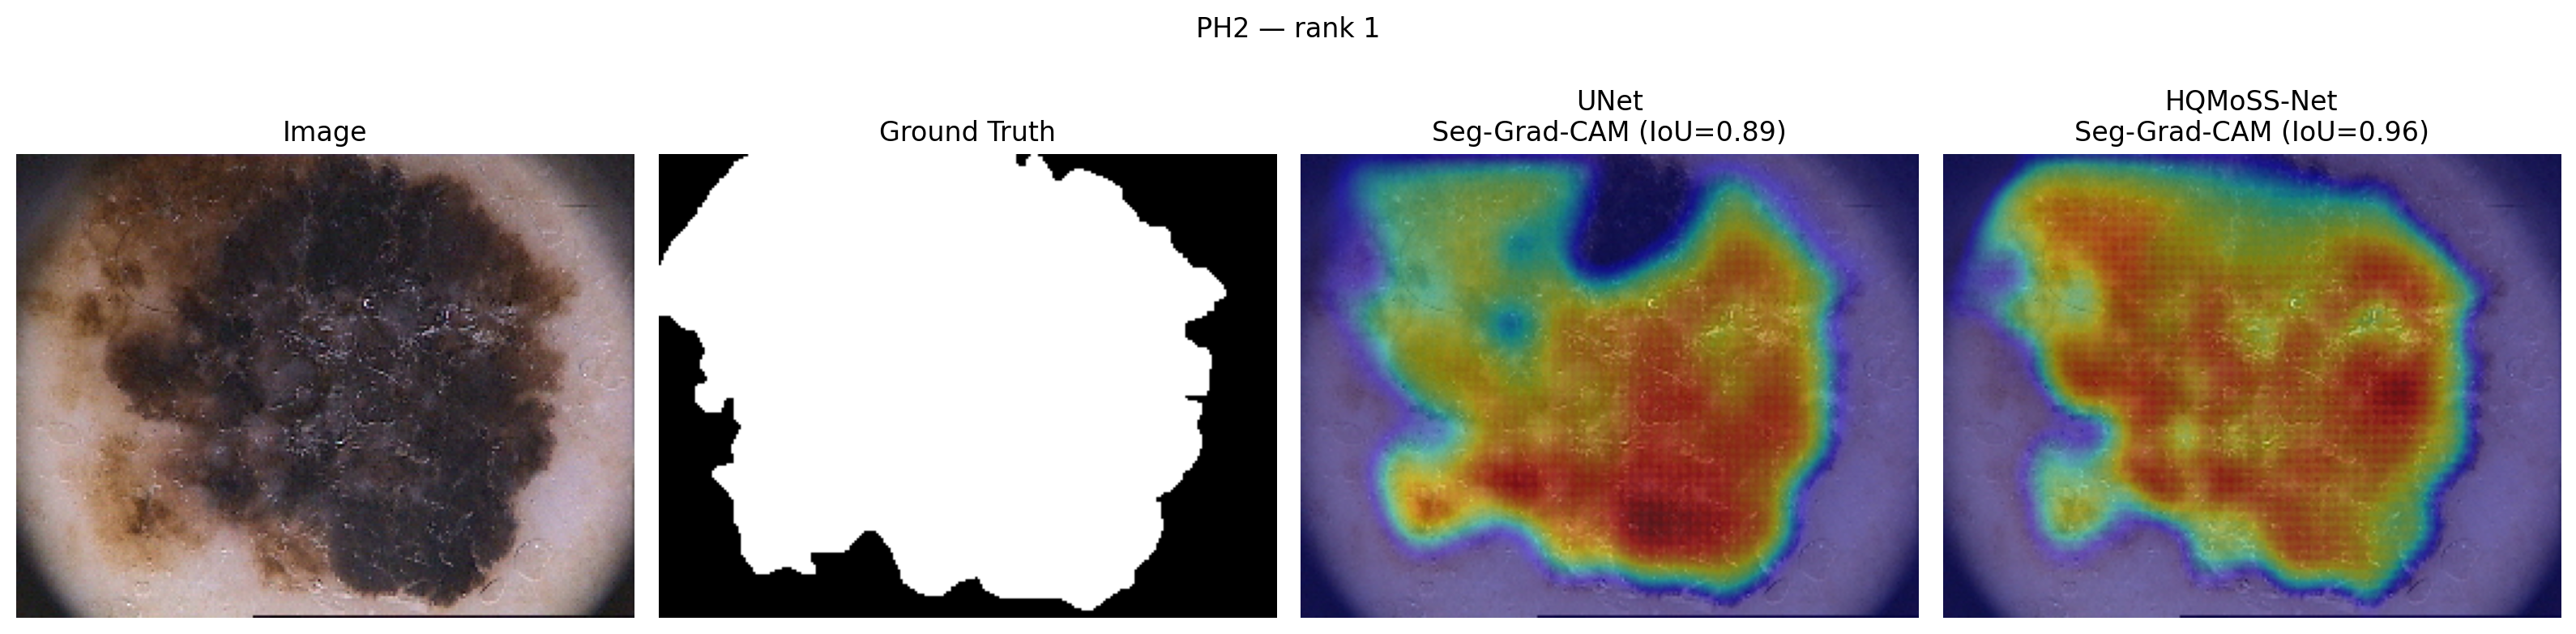
\includegraphics[width=\textwidth]{images/xai_cmp_ph2_1.png}\\[3pt]
    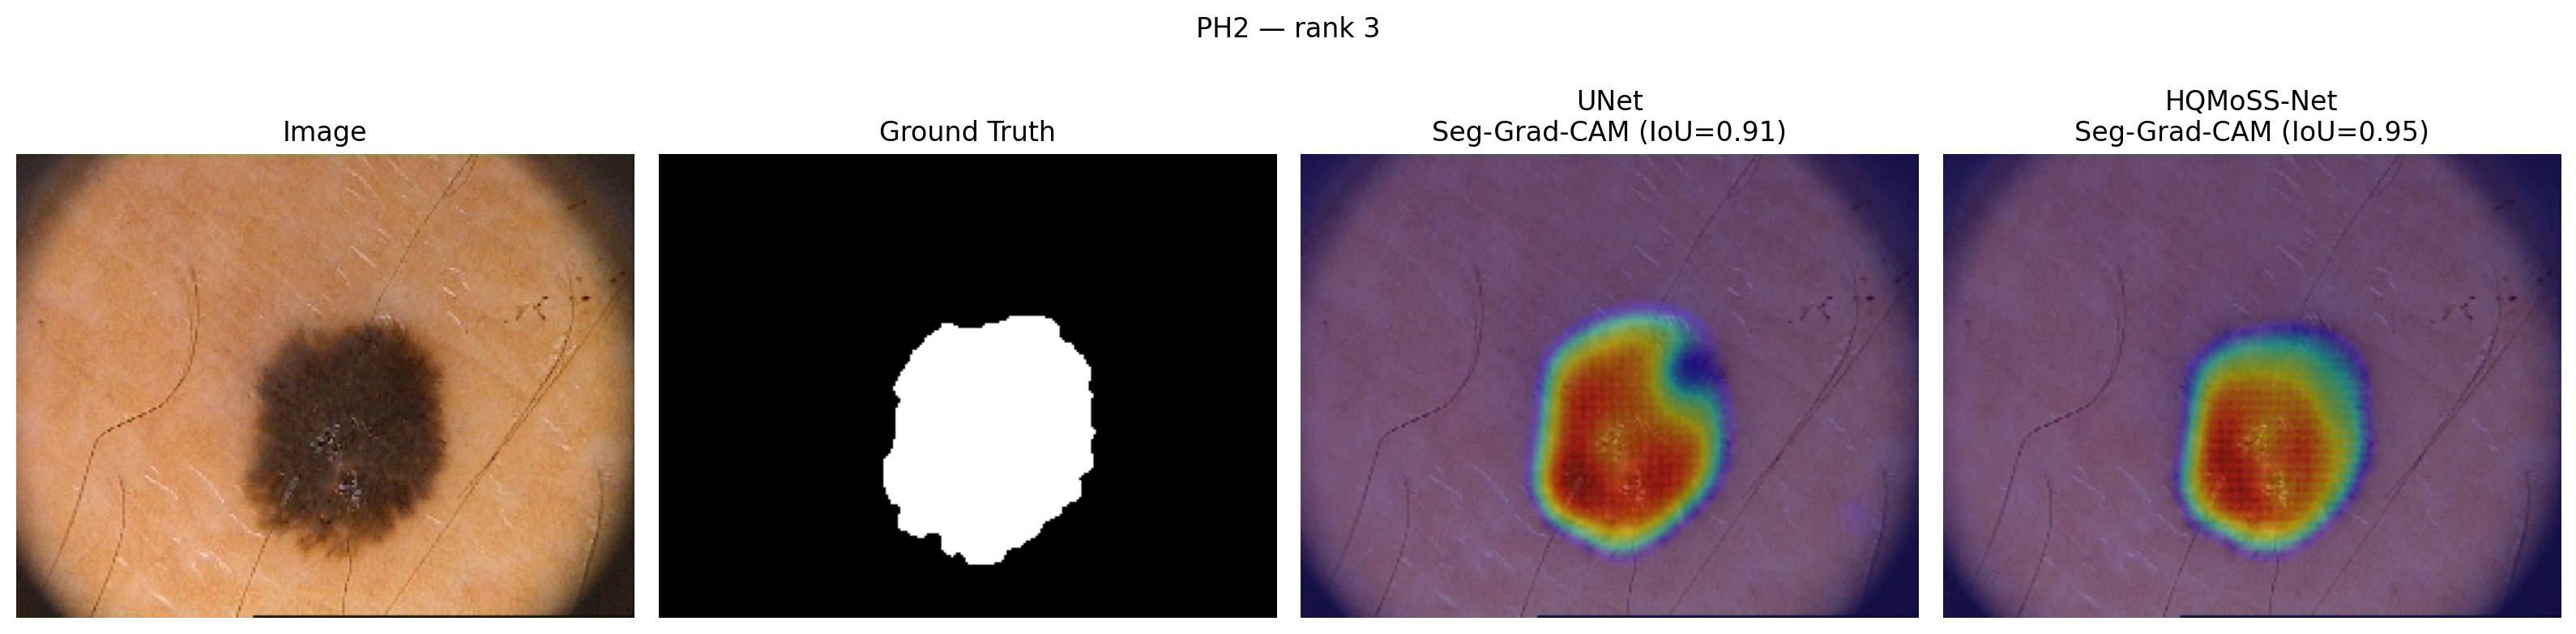
\includegraphics[width=\textwidth]{images/xai_cmp_ph2_2.png}\\[3pt]
    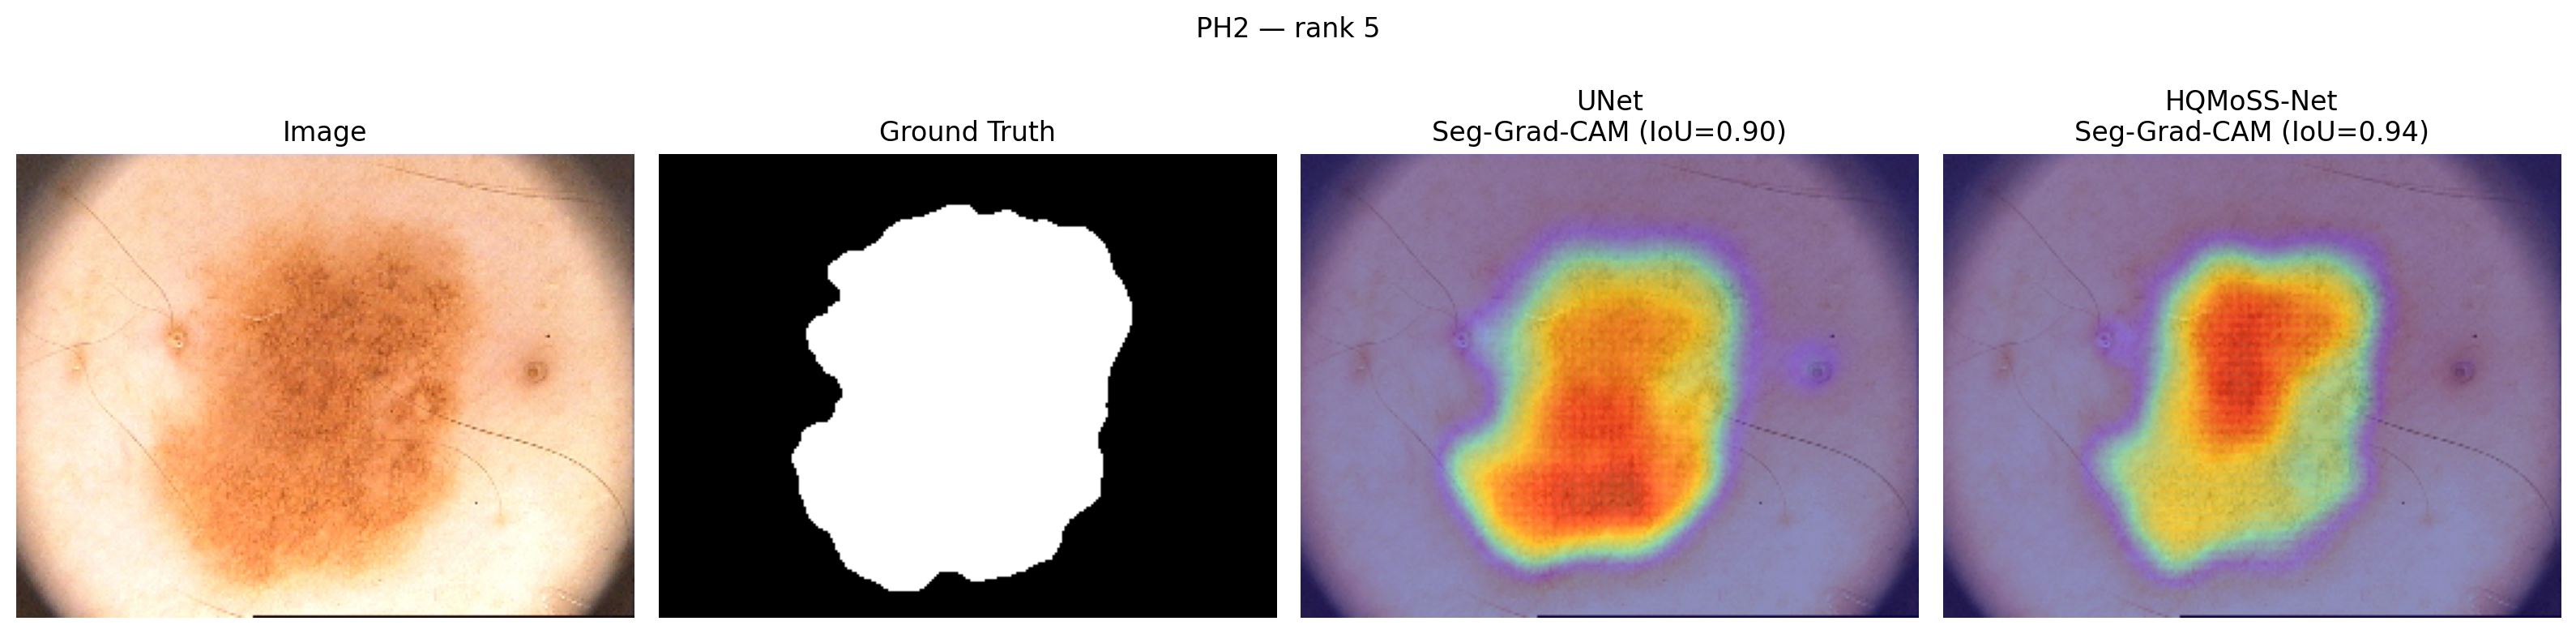
\includegraphics[width=\textwidth]{images/xai_cmp_ph2_3.png}
    \caption{So sánh Seg-Grad-CAM trên PH2. Mỗi hàng, từ trái sang phải: ảnh gốc, mặt nạ thực, bản đồ nhiệt của U-Net và của HQMoSS-Net (kèm IoU matched). Bản đồ nhiệt của HQMoSS-Net bám sát vùng tổn thương hơn hẳn U-Net.}
    \label{fig:seggradcam_compare}
\end{figure}

\begin{figure}[htb!]
    \centering
    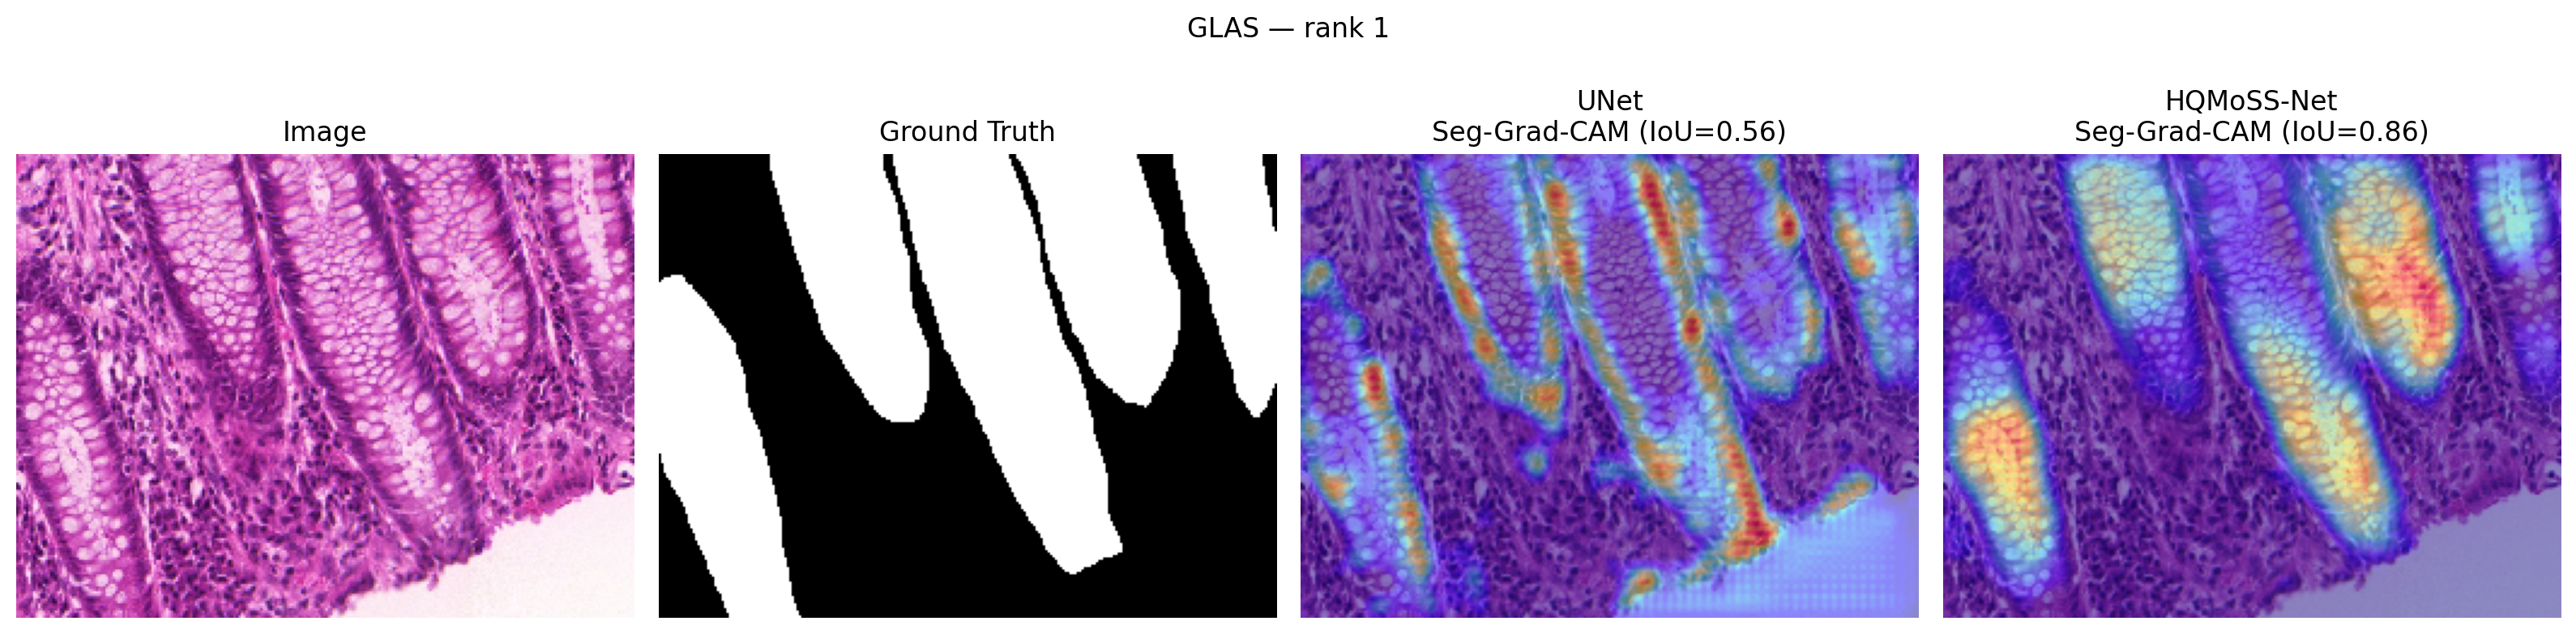
\includegraphics[width=\textwidth]{images/xai_cmp_glas_1.png}\\[3pt]
    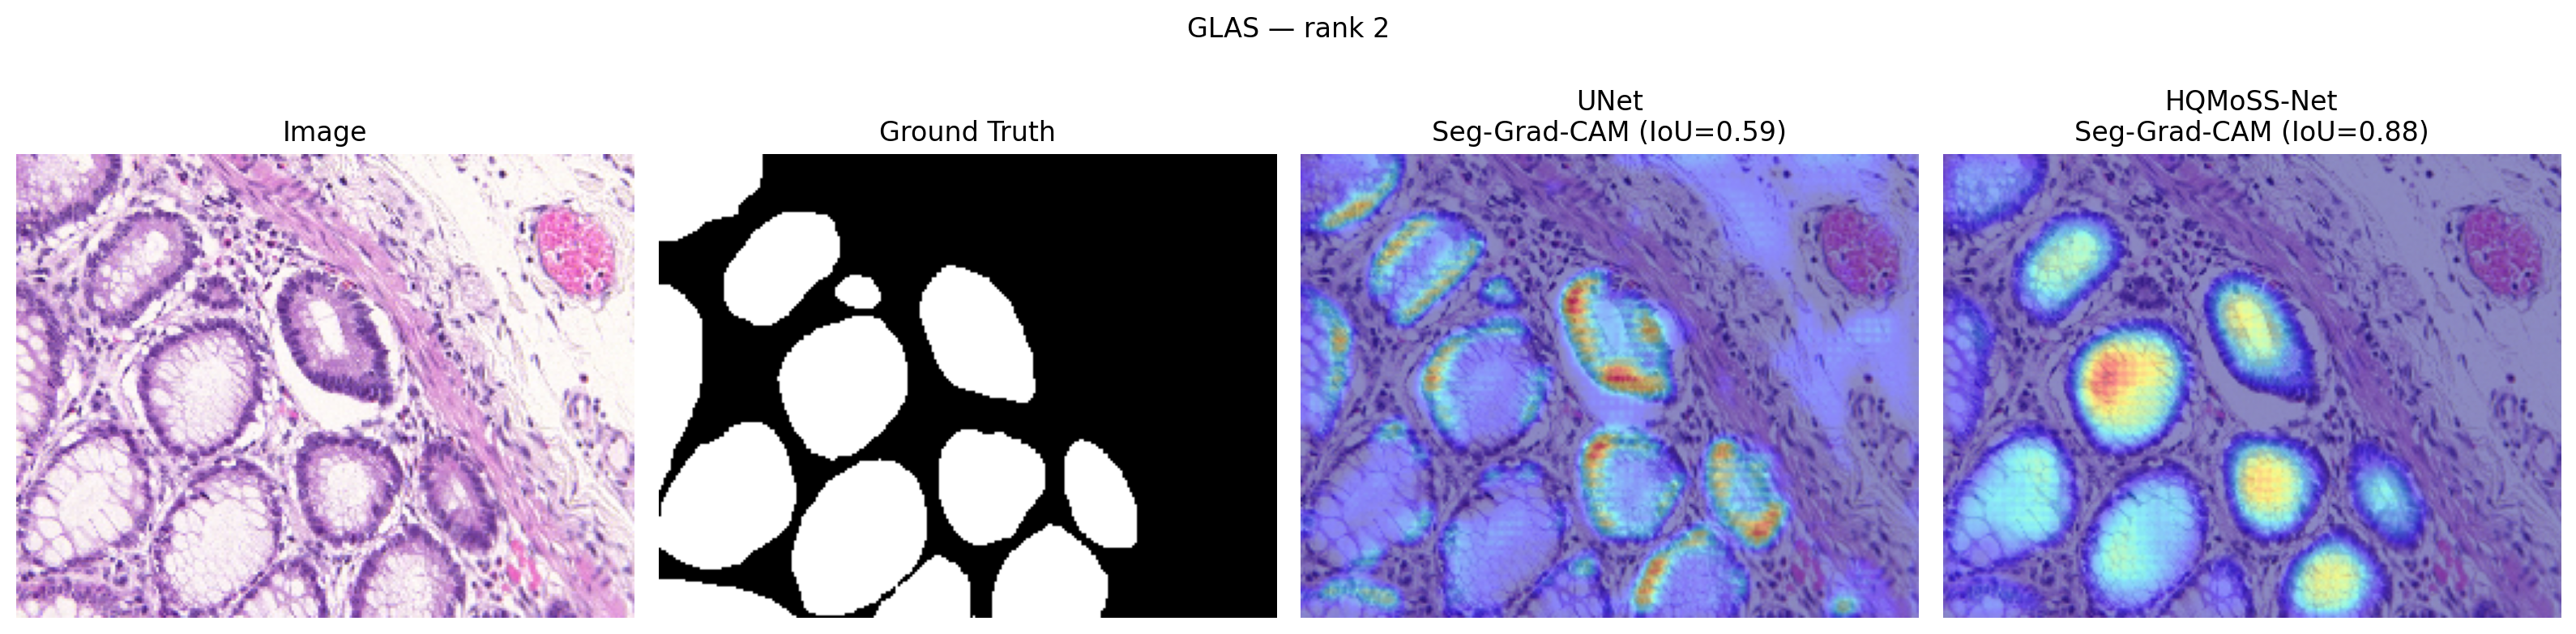
\includegraphics[width=\textwidth]{images/xai_cmp_glas_2.png}\\[3pt]
    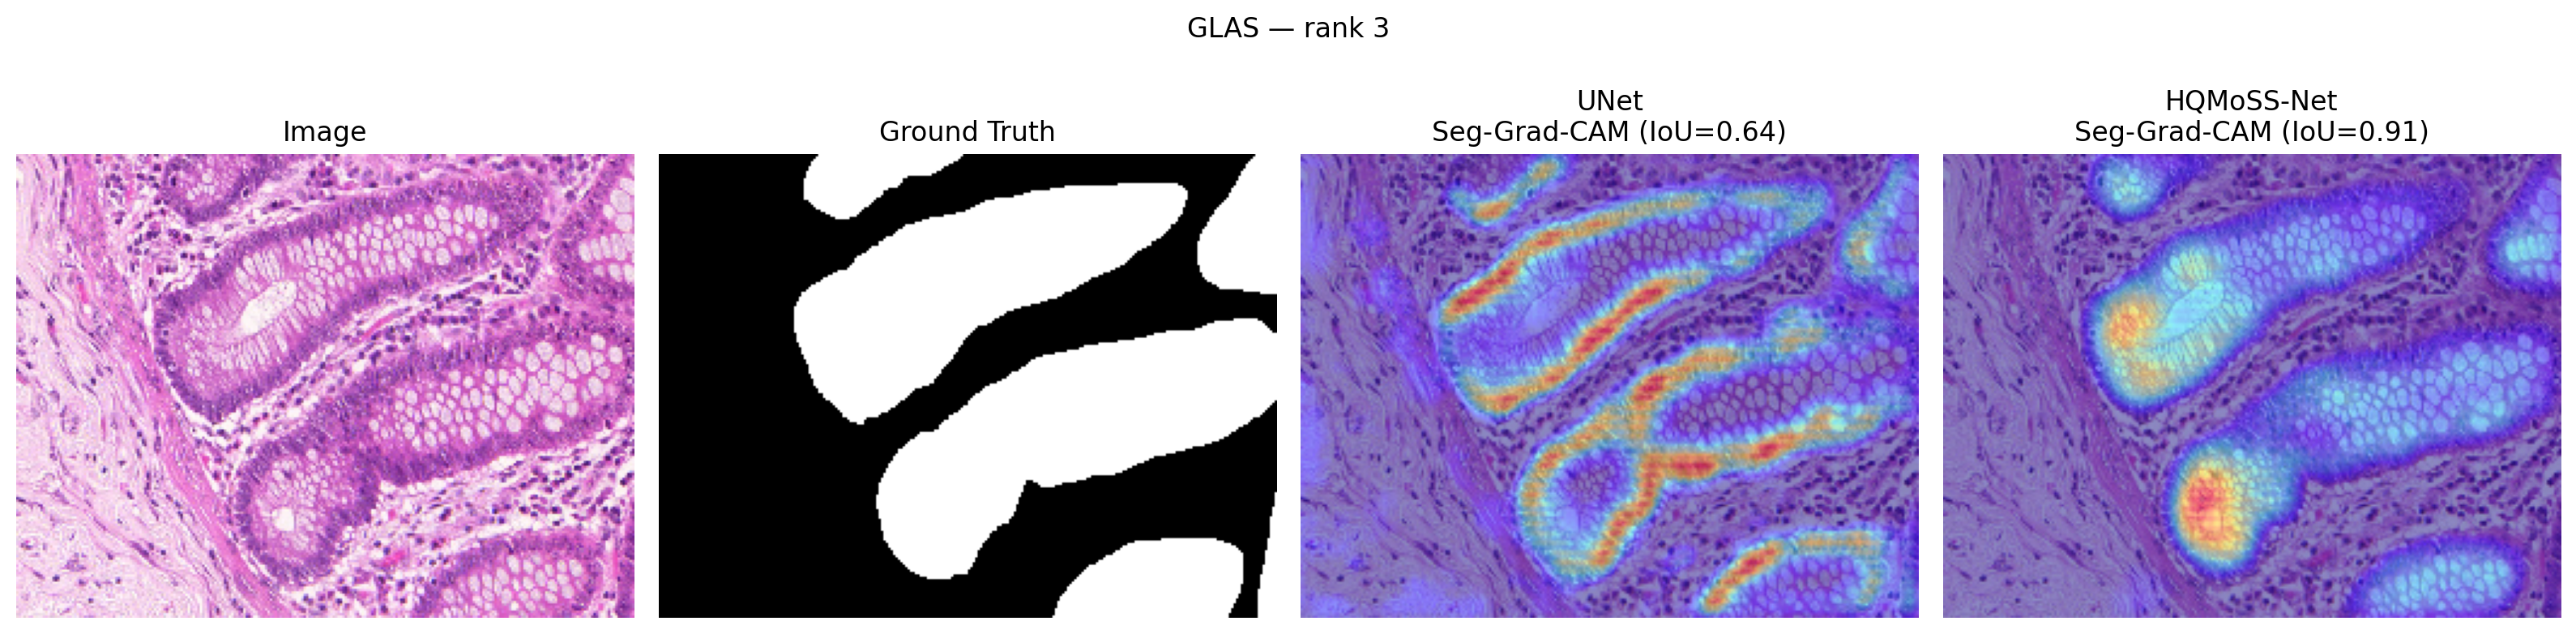
\includegraphics[width=\textwidth]{images/xai_cmp_glas_3.png}
    \caption{So sánh Seg-Grad-CAM trên GlaS 2015 (mô học nhiều tuyến). Mỗi hàng, từ trái sang phải: ảnh gốc, mặt nạ thực, bản đồ nhiệt của U-Net và của HQMoSS-Net (kèm IoU matched). HQMoSS-Net tách và bám các tuyến rời rạc tốt hơn.}
    \label{fig:seggradcam}
\end{figure}

\FloatBarrier

\section{Thảo luận}
Kết quả thực nghiệm cho phép rút ra ba nhận định chính. Thứ nhất, các khối lượng tử góp phần cải thiện chất lượng phân đoạn: HQMoSS-Net đạt kết quả cao hơn mọi baseline trên cả hai tập dữ liệu, và mức chênh lệch lớn hơn trên tập khó hơn (GlaS 2015) -- dù đây mới là quan sát trên hai bộ dữ liệu nên chưa đủ cơ sở để khẳng định chắc chắn một xu hướng tổng quát (biểu diễn lượng tử "đặc biệt có giá trị khi bài toán phức tạp"), cần thêm thực nghiệm trên nhiều bộ dữ liệu đa dạng hơn mới kiểm chứng được. Thứ hai, ưu thế này đạt được với \emph{hiệu quả tham số} cao -- mô hình nhỏ hơn UNet++, Attention U-Net, V-Net và R2U-Net nhiều lần nhưng vẫn đạt kết quả cao hơn, đồng thời ổn định hơn (độ lệch chuẩn nhỏ) qua các fold; đối chứng cổ điển ở mục~\ref{subsec:cmoe_vs_qumoe} cho thêm một tín hiệu khiêm tốn củng cố quan sát này, khi một khối cổ điển cùng kiến trúc nhưng nhiều tham số hơn hẳn lại không đạt hiệu năng và độ ổn định tương đương -- dù đây mới là một phép đối chứng đơn lẻ, chưa phải bằng chứng đầy đủ. Thứ ba, phân tích bóc tách cho thấy ba thành phần RDMS, QuMoE và LSS có tính bổ trợ; đồng thời so sánh với QuNet (mốc lượng tử QuFeX) cho thấy cách tổ chức thành phần lượng tử theo hướng Mixture-of-Experts của khóa luận hiệu quả hơn trong thực nghiệm này. Cuối cùng, phân tích Seg-Grad-CAM -- cả định lượng (tính hợp lý và tính trung thực) lẫn định tính -- cho thấy HQMoSS-Net ``nhìn'' đúng vùng đối tượng và bám biên tốt hơn U-Net trên cả hai bộ dữ liệu.

Hạn chế thực tiễn lớn nhất vẫn là chi phí mô phỏng giả lập lượng tử: dù số lần đánh giá mạch đã được kiểm soát ở tầng bottleneck độ phân giải thấp ($61$ lần/ảnh, mục về độ phức tạp ở Chương~\ref{Chapter4}), thời gian huấn luyện vẫn dài hơn đáng kể so với các mô hình cổ điển. Đây là đánh đổi cần cân nhắc và là động lực cho các hướng phát triển ở Chương~\ref{Chapter6}.
